\pdfminorversion=4
\pdfobjcompresslevel=0
\documentclass[ignorenonframetext,]{beamer}
\setbeamertemplate{caption}[numbered]
\setbeamertemplate{caption label separator}{:}
\setbeamercolor{caption name}{fg=normal text.fg}
\usepackage{amssymb,amsmath}
\usepackage{colortbl}
\usepackage{booktabs}
\usepackage{pifont}
\usepackage{graphicx}
\usepackage{ifxetex,ifluatex}
\usepackage{fixltx2e} % provides \textsubscript
\usepackage{lmodern}
\usepackage{pdfpages}
%\setbeamercolor{background canvas}{bg=}
\makeatletter\beamer@ignorenonframefalse\makeatother
% see https://tex.stackexchange.com/questions/96581/incorrect-frame-numbers-when-pages-included-using-pdfpages-in-beamer
\def\getpdfpages#1#2{\begingroup
	\setbeamercolor{background canvas}{bg=}
	\includepdf[pages={#1}, trim=0mm 1mm 0mm 0mm,%
	pagecommand={\global\setcounter{framenumber}{%
			\the\numexpr\value{framenumber}+1\relax}%
		\expandafter\def\expandafter\insertshorttitle\expandafter{%
			\insertshorttitle\hfill\insertframenumber\,/\,\inserttotalframenumber}}%
	]{#2}
	\endgroup}

\ifxetex
  \usepackage{fontspec,xltxtra,xunicode}
  \defaultfontfeatures{Mapping=tex-text,Scale=MatchLowercase}
  \newcommand{\euro}{€}
\else
  \ifluatex
    \usepackage{fontspec}
    \defaultfontfeatures{Mapping=tex-text,Scale=MatchLowercase}
    \newcommand{\euro}{€}
  \else
    \usepackage[T1]{fontenc}
    \usepackage[utf8]{inputenc}
      \fi
\fi
% use upquote if available, for straight quotes in verbatim environments
\IfFileExists{upquote.sty}{\usepackage{upquote}}{}
% use microtype if available
\IfFileExists{microtype.sty}{\usepackage{microtype}}{}
\usepackage{url}

\providecommand{\tightlist}{%
  \setlength{\itemsep}{0pt}\setlength{\parskip}{0pt}}

% Comment these out if you don't want a slide with just the
% part/section/subsection/subsubsection title:
\AtBeginPart{
  \let\insertpartnumber\relax
  \let\partname\relax
  \frame{\partpage}
}
\AtBeginSection{
  \let\insertsectionnumber\relax
  \let\sectionname\relax
  \frame{\sectionpage}
}
\AtBeginSubsection{
  \let\insertsubsectionnumber\relax
  \let\subsectionname\relax
  \frame{\subsectionpage}
}

\setlength{\parindent}{0pt}
\setlength{\parskip}{6pt plus 2pt minus 1pt}
\setlength{\emergencystretch}{3em}  % prevent overfull lines
\setcounter{secnumdepth}{0}
\usepackage[english]{babel}
\usepackage{dsfont}
\usepackage{verbatim}
\usepackage{amsmath}
\usepackage{amssymb}
\usepackage{amsthm}
\usepackage{amsfonts}
\usepackage{csquotes}
\usepackage{multirow}
\usepackage{longtable}
\usepackage{enumerate}
% \usepackage[absolute,overlay]{textpos}
\usepackage{psfrag}
\usepackage{algorithm}
\usepackage{algpseudocode}
\usepackage{eqnarray}
\usepackage{arydshln}
\usepackage{tabularx}
\usepackage{placeins}
\usepackage{tikz}
% see https://tex.stackexchange.com/questions/32918/how-can-i-decrease-spaces-between-equations
%\usepackage{setspace}
\usepackage[nodisplayskipstretch]{setspace}
\setstretch{1.0}
\usetikzlibrary{shapes,arrows,automata,positioning,calc}
\usepackage{subfig}
% \usepackage{paralist}
\usepackage{graphicx}
\usepackage{array}
\usepackage{framed}
\usepackage{excludeonly}
\usepackage{fancyvrb}
\usecolortheme{dove}
% \usefonttheme{serif}
\usepackage{xfrac}
\usepackage{xcolor}
\usepackage{mdframed}
\usepackage{caption}
\captionsetup[figure]{labelformat=empty}
\usepackage{transparent}
\usepackage{bm}

% URL color:
\definecolor{myorange}{RGB}{80,224,176}
% Theme color of metropolis
\definecolor{metropolis_theme_color}{RGB}{38,38,38}
% Upper and lower rules of code chunks
\definecolor{darkblue}{RGB}{38,38,38}
% Font color of footer:
\definecolor{mygrey}{RGB}{240,240,240}

\definecolor{accents}{RGB}{80,224,176}

\usepackage{hyperref}
\hypersetup{
    colorlinks = true,
    linkcolor = {black},
    urlcolor = {accents},
    linkbordercolor = {white}
}


%% %%%%%%%%%%%%%%%%%%%%%%%%%%%%%%%%%%%%%%%%%%%%%%%%%%%%%%%%%%%%%%%
%% METROPOLIS THEME + CUSTOMIZATIONS
%% %%%%%%%%%%%%%%%%%%%%%%%%%%%%%%%%%%%%%%%%%%%%%%%%%%%%%%%%%%%%%%%

%\usetheme{metropolis}
%\usetheme{metropolis}
%\useoutertheme{metropolis}
%\useinnertheme{metropolis}
\setbeamercolor{background canvas}{bg=white}
\AtBeginSection{
  \let\insertsectionnumber\relax
  \let\sectionname\relax
    \begin{frame}[c,plain,noframenumbering]
    \sectionpage
    \small{\tableofcontents[currentsection]}
    \end{frame}
}

% remove space of center enviroment which often occurs around includegraphics produced from knitr plots
% https://tex.stackexchange.com/questions/74212/how-can-i-change-the-whitespace-above-and-below-center
\let\oldcenter\center
\let\oldendcenter\endcenter
\renewenvironment{center}{\setlength\topsep{0pt}\oldcenter}{\oldendcenter}

% reduce margins / border
% \setbeamersize{text margin left=10pt,text margin right=10pt}

% Reduce space between code chunks and code output in rmarkdown beamer presentation: https://stackoverflow.com/questions/35734525/reduce-space-between-code-chunks-and-code-output-in-rmarkdown-beamer-presentatio
%\setlength{\parskip}{0pt}
%\setlength{\OuterFrameSep}{-20pt}
\makeatletter
\preto{\@verbatim}{\parskip=0pt \topsep=0pt \partopsep=0pt}
\makeatother

%% Add LMU template:
%% ---------------------------------------------------------------
%\usepackage{./../../_setup/lmu-lecture}
\usepackage{../../style/lmu-lecture}
%\input{../../style/common.tex}
% \usefonttheme{structurebold}
% \RequirePackage[T1]{fontenc}
% \RequirePackage[scaled=0.92]{helvet}   %% Helvetica for sans serif
% \defbeamertemplate*{frametitle}{lecture}[1][left]
% {
%   \ifbeamercolorempty[bg]{frametitle}{}{\nointerlineskip}%
%   \@tempdima=\textwidth%
%   \advance\@tempdima by\beamer@leftmargin%
%   \advance\@tempdima by\beamer@rightmargin%
%   \begin{beamercolorbox}[sep=0.2cm,#1,wd=\the\@tempdima]{frametitle}
%     \if@tempswa\else\csname beamer@fte#1\endcsname\fi%
%     {\usebeamerfont{frametitle}\rule[-0.5ex]{0pt}{2.3ex}\insertframetitle\par}%
%     \if@tempswa\else\vskip-.2cm\fi% set inside beamercolorbox... evil here...
%   \end{beamercolorbox}%
% }
% \def\beamer@fteright{\vskip0.35cm\advance\leftskip by 1.7cm\advance\rightskip by1.7cm}
% \setbeamertemplate{frametitle continuation}[from second][{\small/~\insertcontinuationcount}]
% % ------------------------------------------------------------------------
% % Geometry
% \setbeamersize{text margin left=0.8cm,text margin right=0.8cm}
% \pgfdeclarehorizontalshading{footlineshade}{4mm}{%
%   color(0pt)=(black);%
%   color(1.0\paperwidth)=(structure!50!black)}
% % redefine \ref (it has been redefined somewhere by the beamerclass)
% \def\lectureref#1{\expandafter\@setref\csname r@#1\endcsname\@firstoftwo{#1}}
% % counter for framenumber for current lecture
% \newcounter{lectureframenumber}
% % adjust framenumbers for lecture (check whether reference is already defined)
% \def\addjustlectureframenumber#1{\ifx#1\relax\else%
%   \addtocounter{lectureframenumber}{-\lectureref{lect:@@\thelecture}}\fi}

% % ------------------------------------------------------------------------
% % Navigation symbols
% \setbeamertemplate{navigation symbols}{}
% % ------------------------------------------------------------------------
% % No head lines
% \defbeamertemplate*{headline}{lecture theme}{}
% \setbeamertemplate{frametitle}{\expandafter\uppercase\expandafter\insertframetitle}








%% Add footer:
%% ---------------------------------------------------------------
\setbeamertemplate{footline}[text line]{%
    \noindent\hspace*{\dimexpr-\oddsidemargin-1in\relax}%
     \colorbox{white}{
     \makebox[\dimexpr\paperwidth-2\fboxsep\relax]{
     \color{black}
     \begin{minipage}[c][4.5ex][c]{0.5\linewidth}
       \secname
     \end{minipage}
     \hfill\begin{minipage}[c][4.5ex][c]{0.5\linewidth}
       \flushright
       \insertframenumber{}~/~\inserttotalframenumber~~
     \end{minipage}
     }}%
  \hspace*{-\paperwidth}
}

%% Add titlegraphic:
%% ---------------------------------------------------------------
% \titlegraphic{
%   \transparent{0.7}
%   \includegraphics[width=5cm]{./../../_setup/images/logos/eds_logo_black.png}
% }

%% %%%%%%%%%%%%%%%%%%%%%%%%%%%%%%%%%%%%%%%%%%%%%%%%%%%%%%%%%%%%%%%
%% NICER CODE BACKGROUND
%% %%%%%%%%%%%%%%%%%%%%%%%%%%%%%%%%%%%%%%%%%%%%%%%%%%%%%%%%%%%%%%%

% Define Shaded if not defined already through knitr:
%\definecolor{shadecolor}{RGB}{228,228,228}
\makeatletter
\@ifundefined{Shaded}{%
\newenvironment{Shaded}{\begin{snugshade}}{\end{snugshade}}%
}{}
\makeatother

\renewenvironment{Shaded}{
  %\vspace{5pt}
  \begin{mdframed}[backgroundcolor=black!8,
                   linecolor=darkblue,
                   rightline=false,
				   leftline=false]}{
  \end{mdframed}}


%% %%%%%%%%%%%%%%%%%%%%%%%%%%%%%%%%%%%%%%%%%%%%%%%%%%%%%%%%%%%%%%%
%% CHANGE URL COLOR
%% %%%%%%%%%%%%%%%%%%%%%%%%%%%%%%%%%%%%%%%%%%%%%%%%%%%%%%%%%%%%%%%

\renewcommand\UrlFont{\color{accents}}
% \hypersetup{
%     colorlinks=true,
%     linkcolor=myorange
% }

%% %%%%%%%%%%%%%%%%%%%%%%%%%%%%%%%%%%%%%%%%%%%%%%%%%%%%%%%%%%%%%%%
%% INCLUDE LATEX MATH + OTHER CUSTOMIZATIONS
%% %%%%%%%%%%%%%%%%%%%%%%%%%%%%%%%%%%%%%%%%%%%%%%%%%%%%%%%%%%%%%%%


% Include latex-math
\DeclareOldFontCommand{\sf}{\normalfont\sffamily}{\mathsf}

% \input{./../../latex-math/basic-math.tex}
% \input{./../../latex-math/basic-ml.tex}
% \input{./../../latex-math/ml-bagging.tex}
% \input{./../../latex-math/ml-boosting.tex}
% \input{./../../latex-math/ml-gp.tex}
% \input{./../../latex-math/ml-mbo.tex}
% \input{./../../latex-math/ml-nn.tex}
% \input{./../../latex-math/ml-svm.tex}
% \input{./../../latex-math/ml-trees.tex}
% \InputIfFileExists{./../../latex-math/ml-lm.tex}{}{}
% \InputIfFileExists{./../../latex-math/ml-automl.tex}{}{}
% Additional commands:
\newcommand{\abs}[1]{\ensuremath{\left| #1 \right|}}
%\renewcommand{\pikN}{\hat{\pi}^\Np} % This collides with z



% basic latex stuff
\newcommand{\pkg}[1]{{\fontseries{b}\selectfont #1}} %fontstyle for R packages
\newcommand{\lz}{\vspace{0.5cm}} %vertical space

\newcommand{\oneliner}[1] % Oneliner for important statements
{\begin{block}{}\begin{center}\begin{Large}#1\end{Large}\end{center}\end{block}}

\let\code=\texttt
\let\proglang=\textsf

\setkeys{Gin}{width=0.9\textwidth}

%% %%%%%%%%%%%%%%%%%%%%%%%%%%%%%%%%%%%%%%%%%%%%%%%%%%%%%%%%%%%%%%%
%% EXERCISE COUNTER
%% %%%%%%%%%%%%%%%%%%%%%%%%%%%%%%%%%%%%%%%%%%%%%%%%%%%%%%%%%%%%%%%

% Command for an automatic exercise counter for the exercise sheets:
\newcounter{Exercise}
\newcommand{\exercise}{
  \stepcounter{Exercise}
  \ifnum \theExercise = 1
    \Large{\textbf{Exercise \theExercise}} \\
  \else
    \vspace{\baselineskip} \Large{\textbf{Exercise \theExercise}} \\
  \fi
}

% Command for an automatic exercise counter for the courses:
\newcounter{CourseExercise}
\newcommand{\oneExercise}{
  \stepcounter{CourseExercise}
    \begin{center}
      \huge{Exercise \Roman{CourseExercise}}
    \end{center}
}
\newcommand{\twoExercises}{
  \stepcounter{CourseExercise}
    \begin{center}
      \huge{Exercise \Roman{CourseExercise} \& \stepcounter{CourseExercise} \Roman{CourseExercise}}
    \end{center}
}
\newcommand{\threeExercises}{
  \stepcounter{CourseExercise}
    \begin{center}
      \huge{Exercise \Roman{CourseExercise}, \stepcounter{CourseExercise} \Roman{CourseExercise} \& \stepcounter{CourseExercise} \Roman{CourseExercise}}
    \end{center}
}

\newcommand{\resetExercises}{\setcounter{CourseExercise}{0}}

\usetikzlibrary{shapes,arrows,automata,positioning,calc,chains,trees, shadows}
\tikzset{
  %Define standard arrow tip
  >=stealth',
  %Define style for boxes
  punkt/.style={
    rectangle,
    rounded corners,
    draw=black, very thick,
    text width=6.5em,
    minimum height=2em,
    text centered},
  % Define arrow style
  pil/.style={
    ->,
    thick,
    shorten <=2pt,
    shorten >=2pt,}
}
\usepackage{subfig}
%\beamerdefaultoverlayspecification{<+->}

\title{Data Science Lifecycle}
\date{}

\begin{document}
% \begin{frame}[plain]
% \titlepage
% \end{frame}


% \begin{frame}[plain]{}
% \phantomsection\label{section}
% \end{frame}

\section{The Data Science Lifecycle}\label{the-data-science-lifecycle}

\begin{frame}{Learning Objectives}
By the end of this session, you should be able to:
\begin{itemize}
\item Understand main phases of the data science lifecycle
\item Recognize key concepts and terminology relevant to each phase
\item Identify appropriate tools or methods for each phase of a data science project
\item Structure and plan an ML workflow with awareness of dependencies and constraints
\end{itemize}

\end{frame}

\begin{frame}{The Data Science Lifecycle}
\phantomsection\label{the-data-science-lifecycle-1}
\textbf{Lifecycle Management}: Process of managing a (product) lifecycle from inception, through engineering, design and manufacturing to deployment and eventual disposal.

\textbf{CRISP-DM (Cross-Industry Standard Process for Data Mining, 1996)}:
A widely used framework that formalizes the iterative process of turning data into knowledge. %\citebutton{Shearer C., The CRISP-DM model (2000)}{https://mineracaodedados.wordpress.com/wp-content/uploads/2012/04/the-crisp-dm-model-the-new-blueprint-for-data-mining-shearer-colin.pdf}

%https://docs.google.com/presentation/d/1RCourH6lXL6sycgT6HbIXWb7rnQvA5HJ/edit?slide=id.p1#slide=id.p1
% \begin{figure}[h]
% 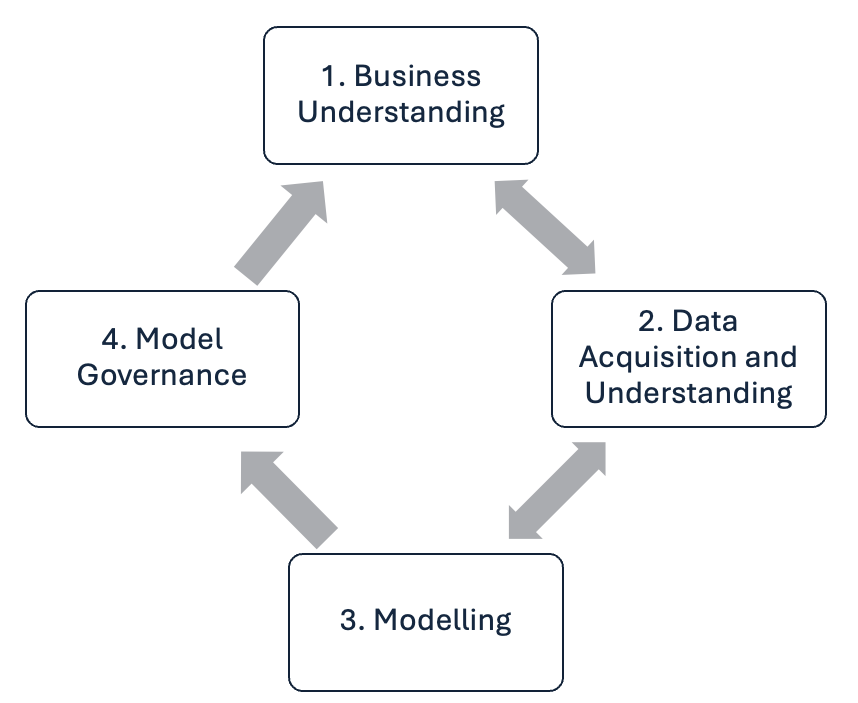
\includegraphics[width=7cm]{figure_man/DSLifecycle1.png}
% \end{figure}

% \end{frame}

% \begin{frame}{The Data Science Lifecycle}
% \phantomsection\label{the-data-science-lifecycle-1}

%https://docs.google.com/presentation/d/1RCourH6lXL6sycgT6HbIXWb7rnQvA5HJ/edit?slide=id.p1#slide=id.p1
\begin{figure}[h]
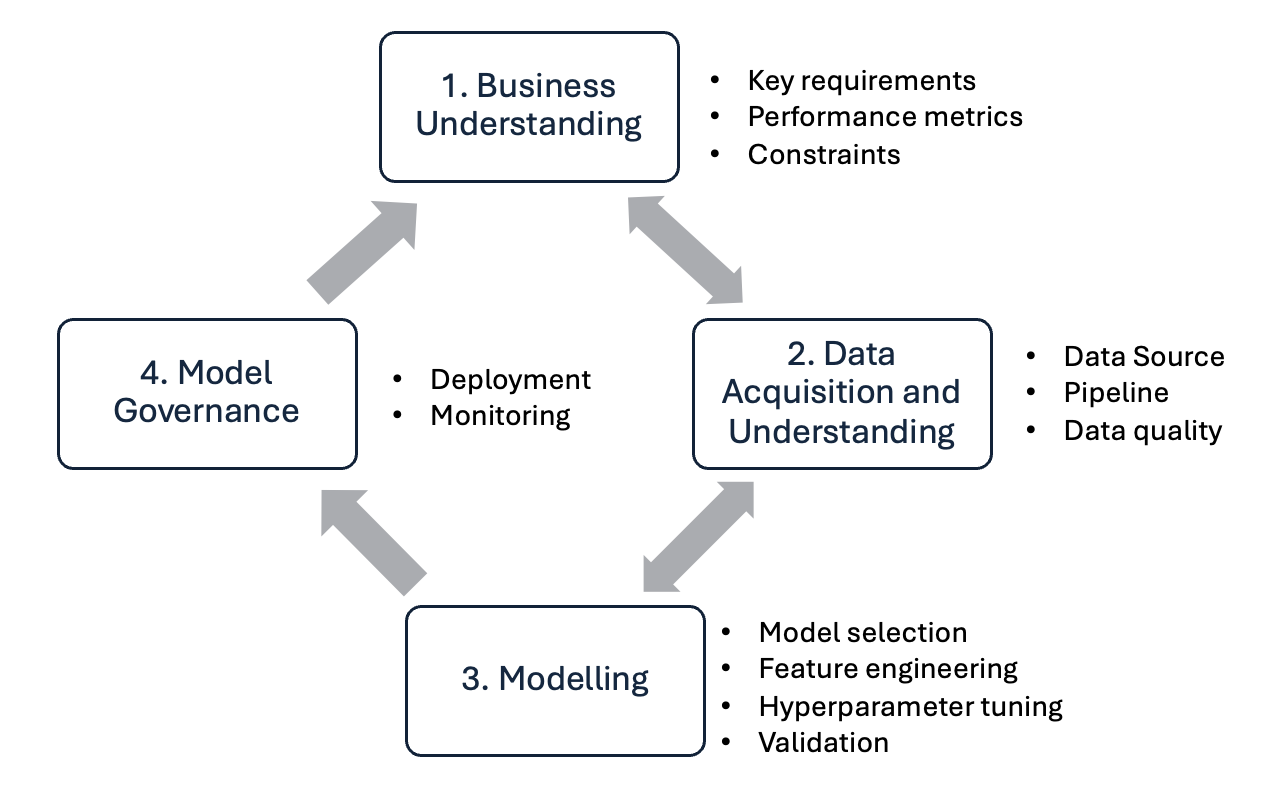
\includegraphics[width=9cm]{figure_man/DSLifecycle2.png}
\end{figure}

\end{frame}


\section{1. Business Understanding}\label{business-understanding-1}

\begin{frame}{Overview Business Understanding}
%https://docs.google.com/presentation/d/1RCourH6lXL6sycgT6HbIXWb7rnQvA5HJ/edit?slide=id.p1#slide=id.p1
\begin{figure}[h]
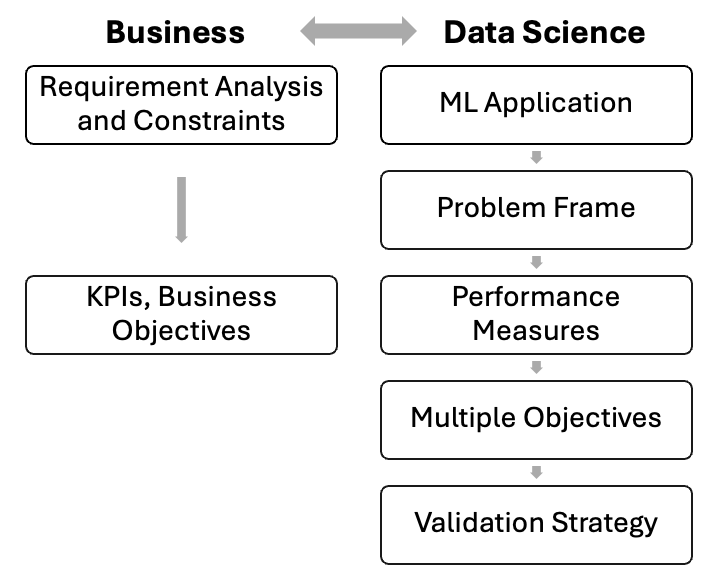
\includegraphics[width=9cm]{figure_man/BusinessUnderstandingOverview.png}
\end{figure}
\end{frame}

\begin{frame}{Requirements Analysis and Constraints}
\phantomsection\label{requirements-analysis}
\textbf{Key question}: What is the end goal of the project?
\begin{itemize}
\tightlist
\item
  Define the intended \textbf{output}:
  \begin{itemize}
  \tightlist
      \item Report, dashboard, or interactive tool?
      \item Scalable pipeline for production use?
  \end{itemize}
\pause
\item Identify constraints% (--> Summarized in \textbf{Service Level Agreements})
    \begin{itemize}
      \tightlist
      \item
        Ethical: Avoid sensitive data use (e.g., address may proxy ethnicity)
      \item
        Legal: Exclude protected attributes (e.g., gender in automated hiring)  %in automated decisions (e.g., job applications).
      \item
        Reproducibility: Ensure the analysis is fully reproducible in a single step
      \item
        Explainability: All model decisions must be explainable to the user
        \item Prediction Latency: Real-time predictions required
        \item Model Size: Stay within specified memory constraints
      \end{itemize}
\end{itemize}
\end{frame}

\begin{frame}{Requirements Analysis and Constraints}
\phantomsection\label{requirements-ml-framing}

\textbf{1. ML Applicability: Is ML justified?}
\begin{itemize}
  \tightlist
  \item Explore non-ML baselines first (rules, heuristics, simple analytics)
  \item Use ML only if patterns are too complex or dynamic
\end{itemize}
\pause
\bigskip
\textbf{2. Problem Framing: How to frame the task?}
\begin{itemize}
  \tightlist
  \item \emph{Imbalanced data:} classification vs.\ anomaly detection?
  \item \emph{Pred. maintenance:} failure probability (classif.) vs.\ remaining lifetime (regr.)?
  \item Select the ML task that aligns with your KPI and data characteristics
\end{itemize}

\vfill
\centering
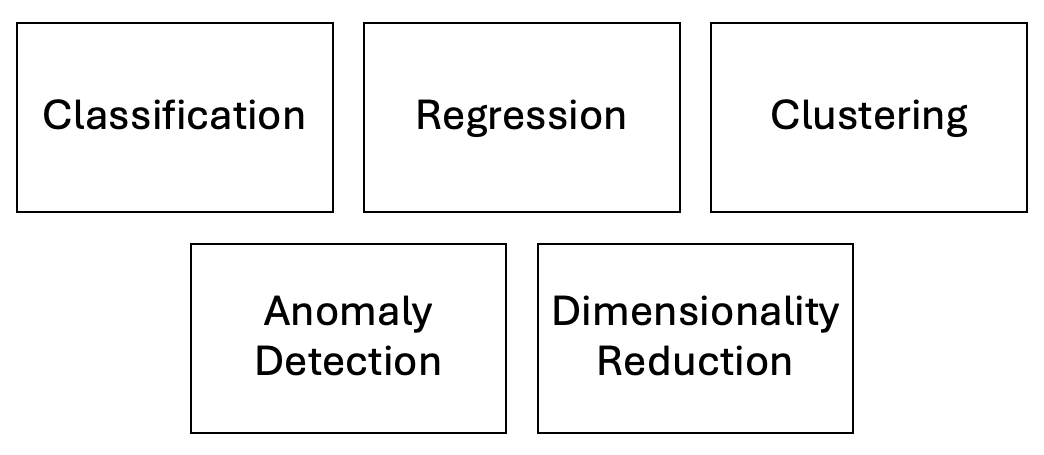
\includegraphics[width=0.6\textwidth]{figure_man/MLTasks.png}
\end{frame}

% \begin{frame}{Requirements Analysis: ML Application}
% \phantomsection\label{non-ml-baseline}
% \textbf{Key question}: Is ML necessary or is a simpler non-ML baseline sufficient?
% \begin{itemize}
% \tightlist
%   \item Consider simpler alternatives first
%   \item Evaluate current rule-based or heuristic systems
%   \item ML is justified when patterns are too complex or dynamic for rules
% \end{itemize}
% \end{frame}

% \begin{frame}{Requirements Analysis: Problem Frame}
% \phantomsection\label{choosing-the-right-problem-frame}
% \textbf{Key question}: Is it classification, regression or something else?
% \begin{itemize}
% \tightlist
% \item
%   A highly imbalanced problem: Frame it as classification, or anomaly
%   detection?
% \item
%   Predictive maintenance: Frame it as classification (probability of
%   failure), or regression (expected remaining lifetime)?
% \item
%   The answer is not clear, but depends on your application. It's
%   important to think about these problems!
% \end{itemize}
% ML-tasks you can select from:
% %https://docs.google.com/presentation/d/1RCourH6lXL6sycgT6HbIXWb7rnQvA5HJ/edit?slide=id.p1#slide=id.p1
% \begin{figure}[h]
% 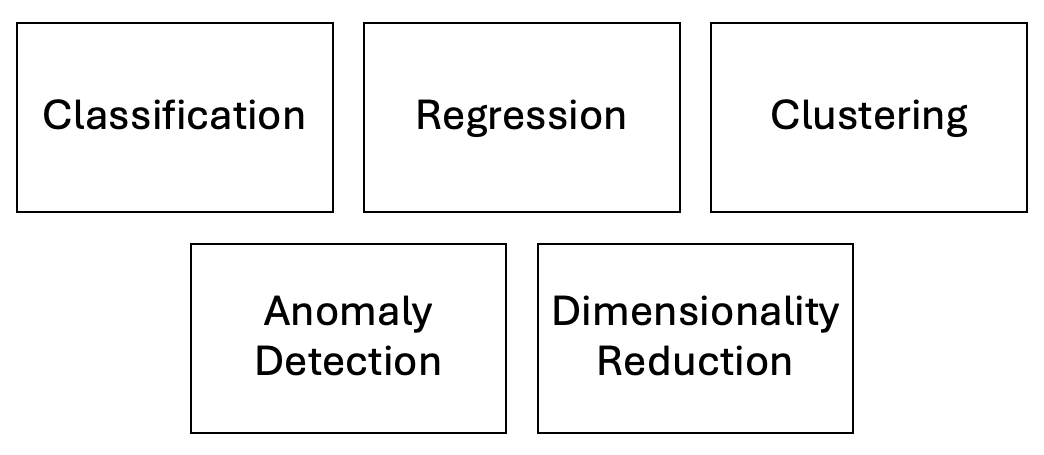
\includegraphics[width=7cm]{figure_man/MLTasks.png}
% \end{figure}
% \end{frame}


% \begin{frame}{KPIs and Business Objectives}
% \phantomsection\label{translating-kpis-into-performance-measures}
% \textbf{KPI}: Key Performance Indicator

% \textbf{Key question}: How does the business side measure success/ performance of the ML solution? How can we translate this to a ML performance measure?

% \begin{itemize}
% \tightlist
% \item
%   Spam detection:

% \begin{itemize}
%   \tightlist
%   \item
%     \emph{Not} OK to misclassify a job application as spam (positive
%     class)
%   \item
%     A spam mail in your inbox once in a while is no problem\\
%     \(\rightarrow\) \emph{minimize the false positive rate},
%     i.e.~maximize precision
%   \end{itemize}
% \item
%   Airport security:

%   \begin{itemize}
%   \tightlist
%   \item
%     \emph{Not} OK to misclassify a weapon (positive class) as laptop
%   \item
%     A false alarm once in a while is no problem\\
%     \(\rightarrow\) \emph{minimize the false negative rate},
%     i.e.~maximize recall
%   \end{itemize}
% \end{itemize}

% \end{frame}

% \begin{frame}{Multiple Objectives}
% \phantomsection\label{multiple-objectives}
% \textbf{Key question}: How to optimize multiple objectives?
% \begin{itemize}
% \tightlist
% \item
%   What if a choice increases objective 1, but decreases objective 2? Is
%   it better?
% \item Maybe maximizing AUC leads to more model complexity and less explainability
% \item
%   There are two common ways to deal with multiple objectives:

%   \begin{itemize}
%   \tightlist
%   \item
%     \textbf{Scalarization} in a \emph{compound measure}:
%     \(obj_1 * obj_2\)
%   \item
%     \textbf{Multi-objective Analysis} %TODO add link for further reading
%   \end{itemize}
% \end{itemize}
% \end{frame}



% \begin{frame}{Performance Measures}
% \phantomsection\label{performance-measures}

% \textbf{Key question}: what performance measure suits best for your solution?

% \begin{itemize}
% \tightlist
%     \item \textbf{Precision and Recall}%: $Precision = \frac{TP}{TP+FP}$, $Recall = \frac{TP}{TP+FN}$
%     \item to capture the tradeoff \textbf{F1-score} $F1 = \frac{2*Recall*Precision}{Recall + Precision}$
%     \item \textbf{Accuracy}: %$Acc = \frac{TP+TN}{TP+TN+FP+FN}$
%     for highly imbalanced data, the accuracy
%   (percentage of correct predictions) is not a good measure
%   \item I.e. in an HIV test, where 99.9\% of the population is healthy, a senseless
%   test that predicts ``healthy'' \emph{all the time}, automatically has
%   an accuracy of 99.9\%
% \end{itemize}

% %https://docs.google.com/presentation/d/1RCourH6lXL6sycgT6HbIXWb7rnQvA5HJ/edit?slide=id.p1#slide=id.p1
% \begin{figure}[h]
% 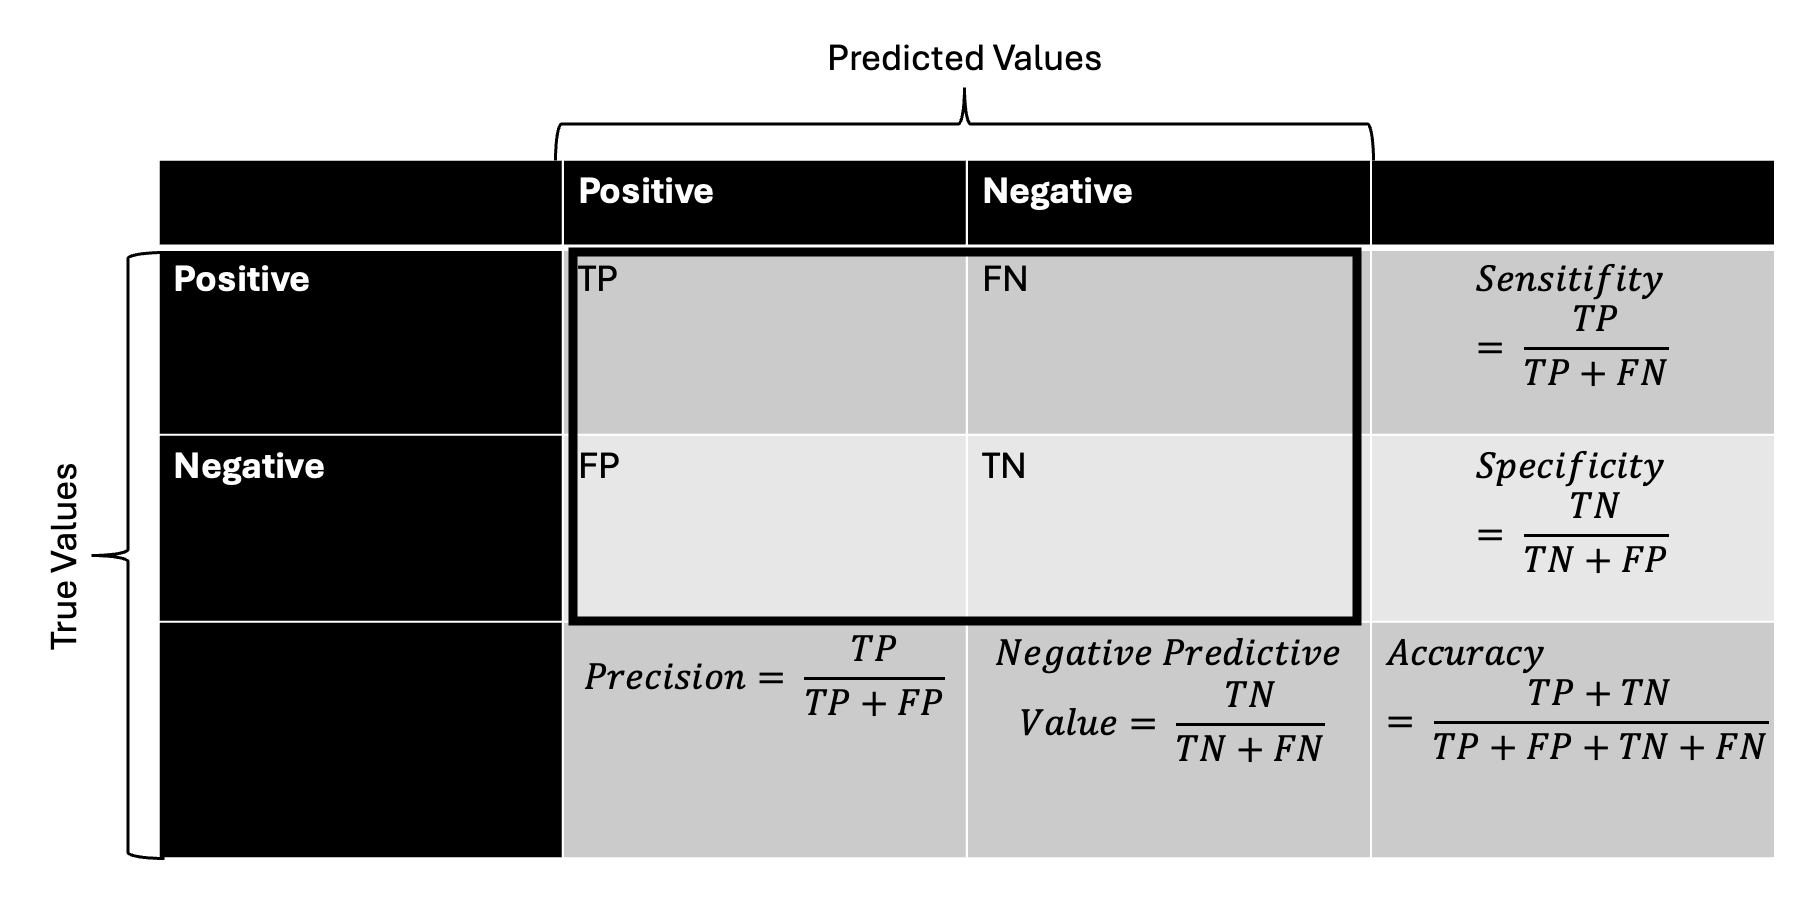
\includegraphics[width=0.72\textwidth]{figure_man/ConfusionMatrix.png}
% \end{figure}
% \end{frame}


\begin{frame}{KPIs \& Business Objectives: Performance Measures}
\phantomsection\label{kpi-metrics-slide}
\vspace{-0.5em}
\begin{itemize}
  \tightlist
  %-----------------------------------------------------------
  \item<1-> \textbf{How to translate key performance indicators (KPIs) to metrics?}
\begin{itemize}
  \tightlist
  \item \textbf{Spam detection}: Job application flagged as spam = unacceptable\\
      $\Rightarrow$ Occasional inbox spam is fine $\Rightarrow$ minimize FP $\Rightarrow$ maximize \textbf{precision}
  \item \textbf{Airport security}:  Weapon flagged as laptop = unacceptable\\
      $\Rightarrow$ Occasional false alarm is fine $\Rightarrow$ minimize FN $\Rightarrow$ maximize \textbf{recall}
\end{itemize}

\only<1>{
    \begin{center}
        
    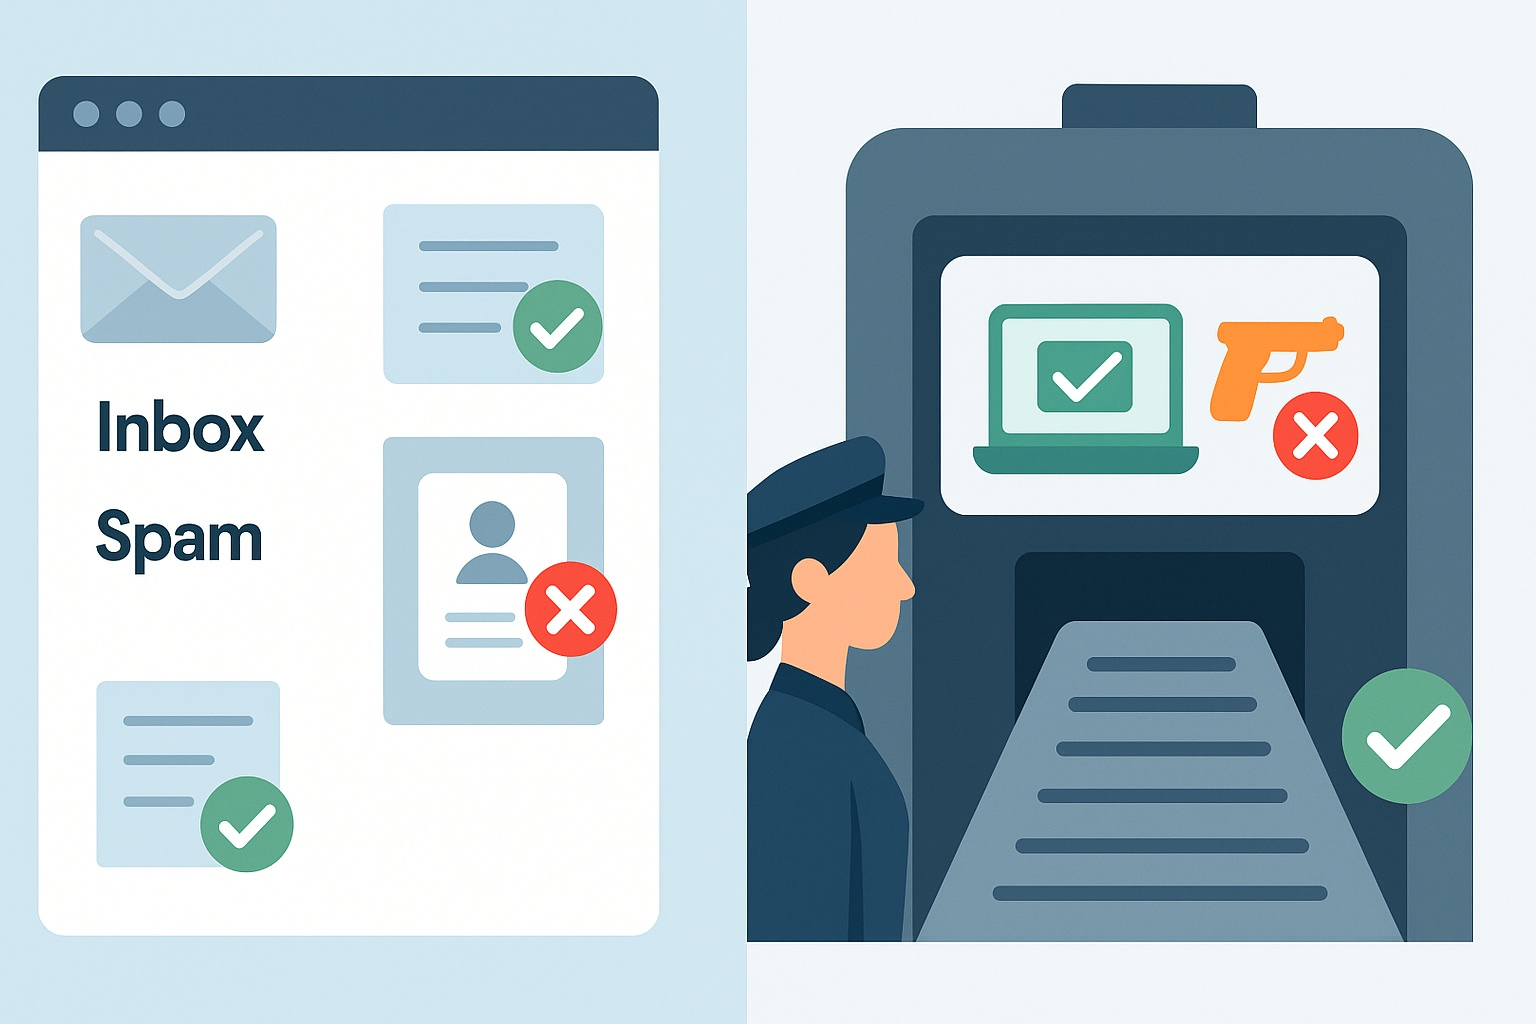
\includegraphics[width=0.5\linewidth]{figure_man/spam_airport.jpg}
    \end{center}
}
  %-----------------------------------------------------------
  \item<2-> \textbf{How to handle multiple objectives?}
    \begin{itemize}
      \tightlist
      \item \textit{Scalarization}: Combine into one score (e.g.\ $F_1$, cost‐weighted loss)
      \item \textit{Pareto/frontier}: Analyze trade-off without collapsing (e.g., ROC curve)
    \end{itemize}
  %-----------------------------------------------------------
  %\item \textbf{Core performance metrics}
    % \begin{itemize}
    %   \tightlist
    %   \item Precision, Recall, $F_1$
    %   \item Accuracy (misleading on severe class imbalance)
    % \end{itemize}
\end{itemize}

\only<2>{
 \scriptsize
 \renewcommand{\arraystretch}{1.5}
\begin{tabular}{|l|cc|c|}
\hline
\multirow{2}{*}{\textbf{True Values}}
  & \multicolumn{2}{c|}{\textbf{Predicted Values}} & \\%[0.3ex]
  & \textbf{Pos} & \textbf{Neg} & \\[0.3ex]
\hline

\textbf{Pos}
  & \cellcolor[gray]{0.9}\rule{0pt}{3.5ex}TP
  & \cellcolor[gray]{0.9}FN
  & \cellcolor[gray]{0.9}\rule{0pt}{3.5ex}%
    \textbf{Sensitivity/Recall/TPR }%
    $=\dfrac{TP}{TP+FN}$ \\

\textbf{Neg}
  & \cellcolor[gray]{0.9}\rule{0pt}{3.5ex}FP
  & \cellcolor[gray]{0.9}TN
  & \cellcolor[gray]{0.9}\rule{0pt}{3.5ex}%
    \textbf{Specificity }%
    $=\dfrac{TN}{TN+FP}$ \\[0.8ex]
\hline
  & \cellcolor[gray]{0.9}\rule{0pt}{3.5ex}
      \textbf{Precision} $=\dfrac{TP}{TP+FP}$
  & \cellcolor[gray]{0.9}\rule{0pt}{3.5ex}
      \textbf{NPV} $=\dfrac{TN}{TN+FN}$
  % & \cellcolor[gray]{0.9}\rule{0pt}{3ex}%
  %     \textbf{Precision} $=\dfrac{TP}{TP+FP}$
  % & \cellcolor[gray]{0.9}\rule{0pt}{3ex}%
  %     \textbf{NPV} $=\dfrac{TN}{TN+FN}$
  & \cellcolor[gray]{0.9}\rule{0pt}{3.5ex}
      \textbf{F$_1$}%
        $=\dfrac{2\,\text{Precision}\,\text{Recall}}%
                {\text{Precision}+\text{Recall}}$
  %\shortstack[l]{%
      %\tiny\rule{0pt}{3.5ex}\textbf{Accuracy }%
      %  $=\dfrac{TP+TN}{TP+FP+TN+FN}$\\[0.8ex]
      %\tiny\rule{0pt}{3ex}\textbf{F$_1$}%
      %  $=\dfrac{2\,\text{Precision}\,\text{Recall}}%
      %          {\text{Precision}+\text{Recall}}$} 
                \\[0.8ex]
\hline
\end{tabular}
}


%\vspace{0.5em}
% \centering
% 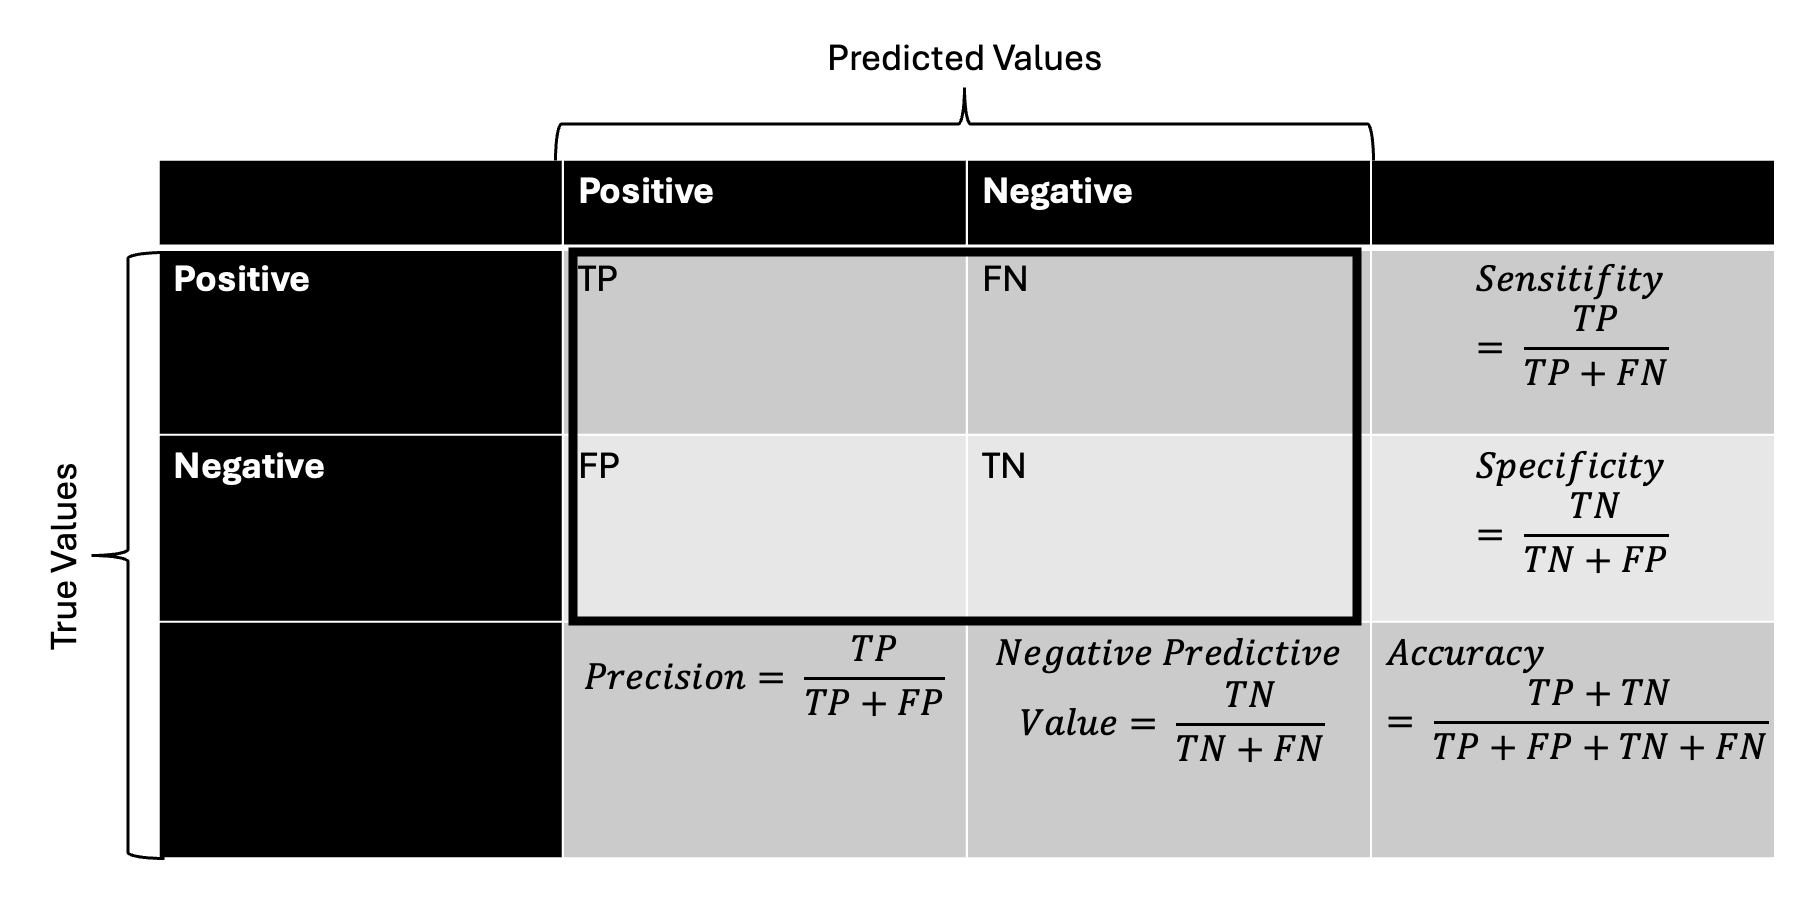
\includegraphics[width=0.65\textwidth]{figure_man/ConfusionMatrix.png}
\end{frame}


% \begin{frame}{Validation Strategy}
% \phantomsection\label{validation-strategy}

% \textbf{Key question}: How to validate the model?

% %from I2ML: https://drive.google.com/file/d/16O-rVIPJVpLIZ9-qb7BRIJxomCXcrNgL/edit
% \begin{figure}[h]
% 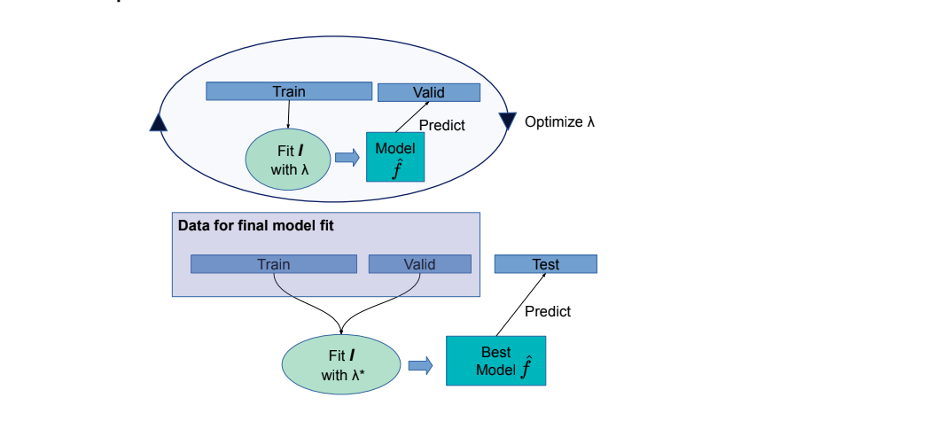
\includegraphics[width=12cm]{figure_man/Validation.png}
% \end{figure}
% \end{frame}

% \begin{frame}{Validation Strategy}
% \phantomsection\label{validation-strategy}

% \textbf{Key question}: How to validate the model?

% Considerations when deciding for a validation strategy:

% \begin{itemize}
% \tightlist
% \item
%   What to generalize to?

%   \begin{itemize}
%   \tightlist
%   \item
%     blocking factors
%   \item
%     temporal effects
%   \item
%     spatial effects
%   \end{itemize}
% \item
%   Validate it just like you would use it in real life:
%   \begin{itemize}
%   \tightlist
%   \item
%     A time series model: You'd build it in 2020 with data from
%     2016--2020, then use it in 2021
%   \item
%     Validate it with the same strategy: Train on 2016--2019, validate on
%     2020
%   \end{itemize}
% \end{itemize}

% \end{frame}

% \begin{frame}{Validation Strategy}
% \phantomsection\label{validation-strategy}

% \textbf{Key question}: How to validate the model?

% be aware of \textbf{data leakage}
% \begin{itemize}
% \tightlist
%     \item Target Leakage: When features that won’t be available at prediction time contain information about the target variable.
%     \begin{itemize}
%     \tightlist
%         \item Example: Using "Total Sales in Next Month" as a predictor when trying to forecast sales.
%     \end{itemize} 
%     \item Train-Test Leakage: 
%     \begin{itemize}
%     \tightlist
%         \item Example: Normalizing the dataset using the entire data before splitting into train and test sets.
%     \end{itemize}
% \end{itemize}
% \end{frame}


\begin{frame}{KPIs \& Business Objectives: Validation Strategy}
\phantomsection\label{validation-strategy}

\textbf{Key question}: How to validate the model reliably and realistically?

\textbf{Part 1: Strategic Considerations}
\begin{itemize}
  \item \textbf{What should your model generalize to?}
    \begin{itemize}
      \item \emph{Blocking factors} (e.g., customers, hospitals, product types)
      \item \emph{Temporal effects} (e.g., seasonality, trends)
      \item \emph{Spatial effects} (e.g., regions, branches)
    \end{itemize}

  \item \textbf{Simulate realistic deployment:}
    \begin{itemize}
      \item \textbf{Time series:} Train on data from 2016--2020, deploy in 2021
  \item \textbf{Validation:} Mimic deployment -- train on 2016--2019, validate on 2020
      % \item Time series: Train on 2016--2019, validate on 2020, deploy in 2021
      % \item Match your validation logic to your intended use case
    \end{itemize}
\end{itemize}

\only<1>{
    \begin{center}
        
    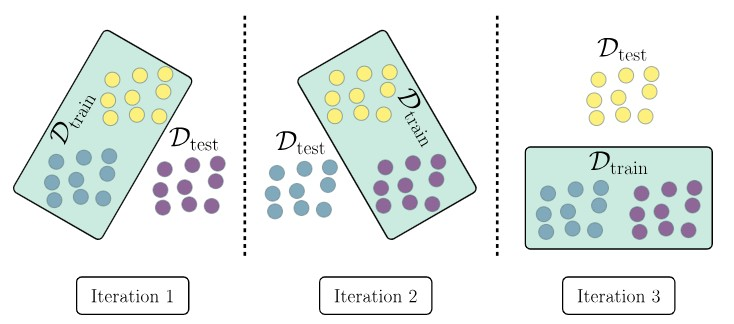
\includegraphics[width=0.5\linewidth]{figure_man/blocking.jpg}
    \end{center}
}
\only<2>{
\vspace{0.5em}
\textbf{Part 2: Beware of Data Leakage}
\begin{itemize}
  \item \textbf{Target Leakage:} Features leak future information not available at prediction time
    \begin{itemize}
      \item Example: "Total Sales in Next Month" used to predict this month
    \end{itemize}

  \item \textbf{Train-Test Leakage:} Information from the test set is used during training
    \begin{itemize}
      \item Example: Scaling the full dataset before splitting
    \end{itemize}
\end{itemize}
}
%\textbf{Guideline:} Always split your data first, then apply transformations only on training folds.
\end{frame}





% \section{2. Data Acquisition and
% Understanding}\label{data-acquisition-and-understanding-1}

% \begin{frame}{Data Source}
% \phantomsection\label{data-source}
% \textbf{Key question}: Where does the data come from?

% In real world, there are multiple data sources

% \begin{minipage}{0.3\textwidth}
% %https://docs.google.com/presentation/d/1RCourH6lXL6sycgT6HbIXWb7rnQvA5HJ/edit?slide=id.p1#slide=id.p1
% 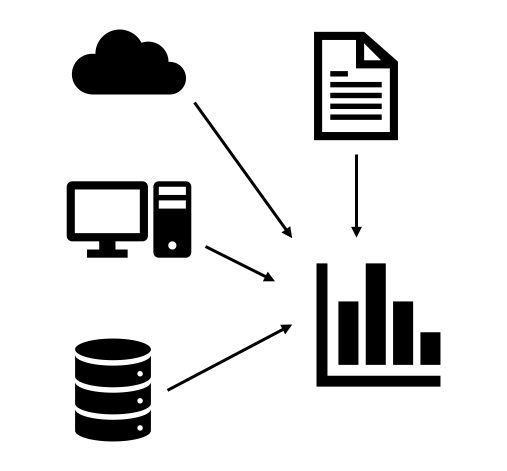
\includegraphics[width=\linewidth]{figure_man/DataSources.png}
% \end{minipage}
% \begin{minipage}{0.6\textwidth}%\RaggedRight
% \begin{itemize}
% %\tightlist
%     \item \textbf{internal vs. external data sources}: external providers might change their data format or discontinue the service
%     \item \textbf{structured vs. unstructured}: structured data can be stored in a database, unstructured one might include images and is not so straightforward to work with
%     \item \textbf{database vs. files}: databases combine many advantages of other file types, most software can grab and process data from there.
%     \item \textbf{on-premise vs. cloud:} decision depends on data protection laws, costs and team preferences
% \end{itemize}
% \end{minipage}

% \end{frame}

\section{2. Data Acquisition and Understanding}\label{data-acquisition-and-understanding}

\begin{frame}{Data Sources}
\phantomsection\label{data-source}
\textbf{Key question:} What data is available and where does it come from?

\bigskip
\begin{columns}[T]
  \begin{column}{0.35\textwidth}
    \centering
    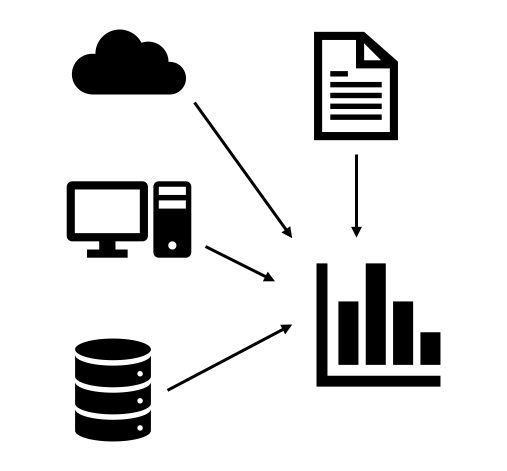
\includegraphics[width=\linewidth]{figure_man/DataSources.png}
  \end{column}

  \begin{column}{0.60\textwidth}
    \begin{itemize}
      \tightlist
      \item \textbf{Internal vs. External:} External feeds may change format or be discontinued
      \item \textbf{Structured vs. Unstructured:} Tables vs.\ free-text, images, audio, etc.
      \item \textbf{Databases vs. Files:} DBs offer querying, consistency and security
      \item \textbf{On-Premise vs. Cloud:} Governed by regulations, cost and team expertise
    \end{itemize}
  \end{column}
\end{columns}
\end{frame}


% \begin{frame}{Data Access at Deployment Time}
% \phantomsection\label{data-access-at-deployment-time}
% \textbf{Key question}: How to feed the \emph{new} data to your model when it's in use?
% \begin{itemize}
% \tightlist
% \item
%   This is often a separate workflow than your training data pipeline
% \item
%   Plan ahead: Think about these questions in the beginning
% \end{itemize}
% \end{frame}

\begin{frame}{Data Exploration}
\phantomsection\label{data-exploration}
\textbf{Key question}: What are the data features and how do they look like?
\begin{itemize}
\tightlist
\item Create a \emph{data dictionary} to clarify:

  \begin{itemize}
  \tightlist
\item Semantic meaning of each feature
    \item Measurement units and expected ranges
    \item Valid levels for categorical features (factors)
    \item Encoding scheme for missing or special values
  \end{itemize}
\item  Compute (stratified) summary statistics and inspect missingness
\item  Plot uni- and bivariate diagrams to explore distributions and structure
  \item Identify:
  \begin{itemize}
    \item Outliers, anomalies, imbalances
    \item Redundant or highly correlated features
  \end{itemize}
\end{itemize}
\end{frame}

\begin{frame}{Data Quality}
\phantomsection\label{data-quality}
\textbf{Key question:} Is the data fit for modeling? \emph{Garbage in, garbage out.}

\begin{itemize}
  \item Assess missingness: How many values are missing, and where?
  \item Detect implausible or inconsistent values (requires domain expertise)
  \item Standardize formats (e.g., date/time parsing)
  \item Drop near-constant or non-informative features
  \item Remove redundancy and obsolete variables
\end{itemize}

\vspace{0.5em}
\textbf{Watch for data bias:}
\begin{itemize}
  \item \textit{Sampling bias:} E.g., a survey at 10am in the city center misses working adults
  \item \textit{Response bias:} Online reviews often reflect extreme opinions, not the median
\end{itemize}
\end{frame}



\begin{frame}{Datasheets}
\phantomsection\label{datasheets}
\href{https://arxiv.org/abs/1803.09010}{Gebru et al., 2018 — Datasheets for Datasets}

\emph{Datasheets} summarize key metadata about a dataset’s content, structure, provenance, and known limitations to support informed and responsible use.

  \begin{itemize}
    \item Why and how was the data collected?
    \item What are its limitations and ethical concerns?
    \item For which tasks is it suitable or unsuitable?
  \end{itemize}

\begin{figure}
    \centering
    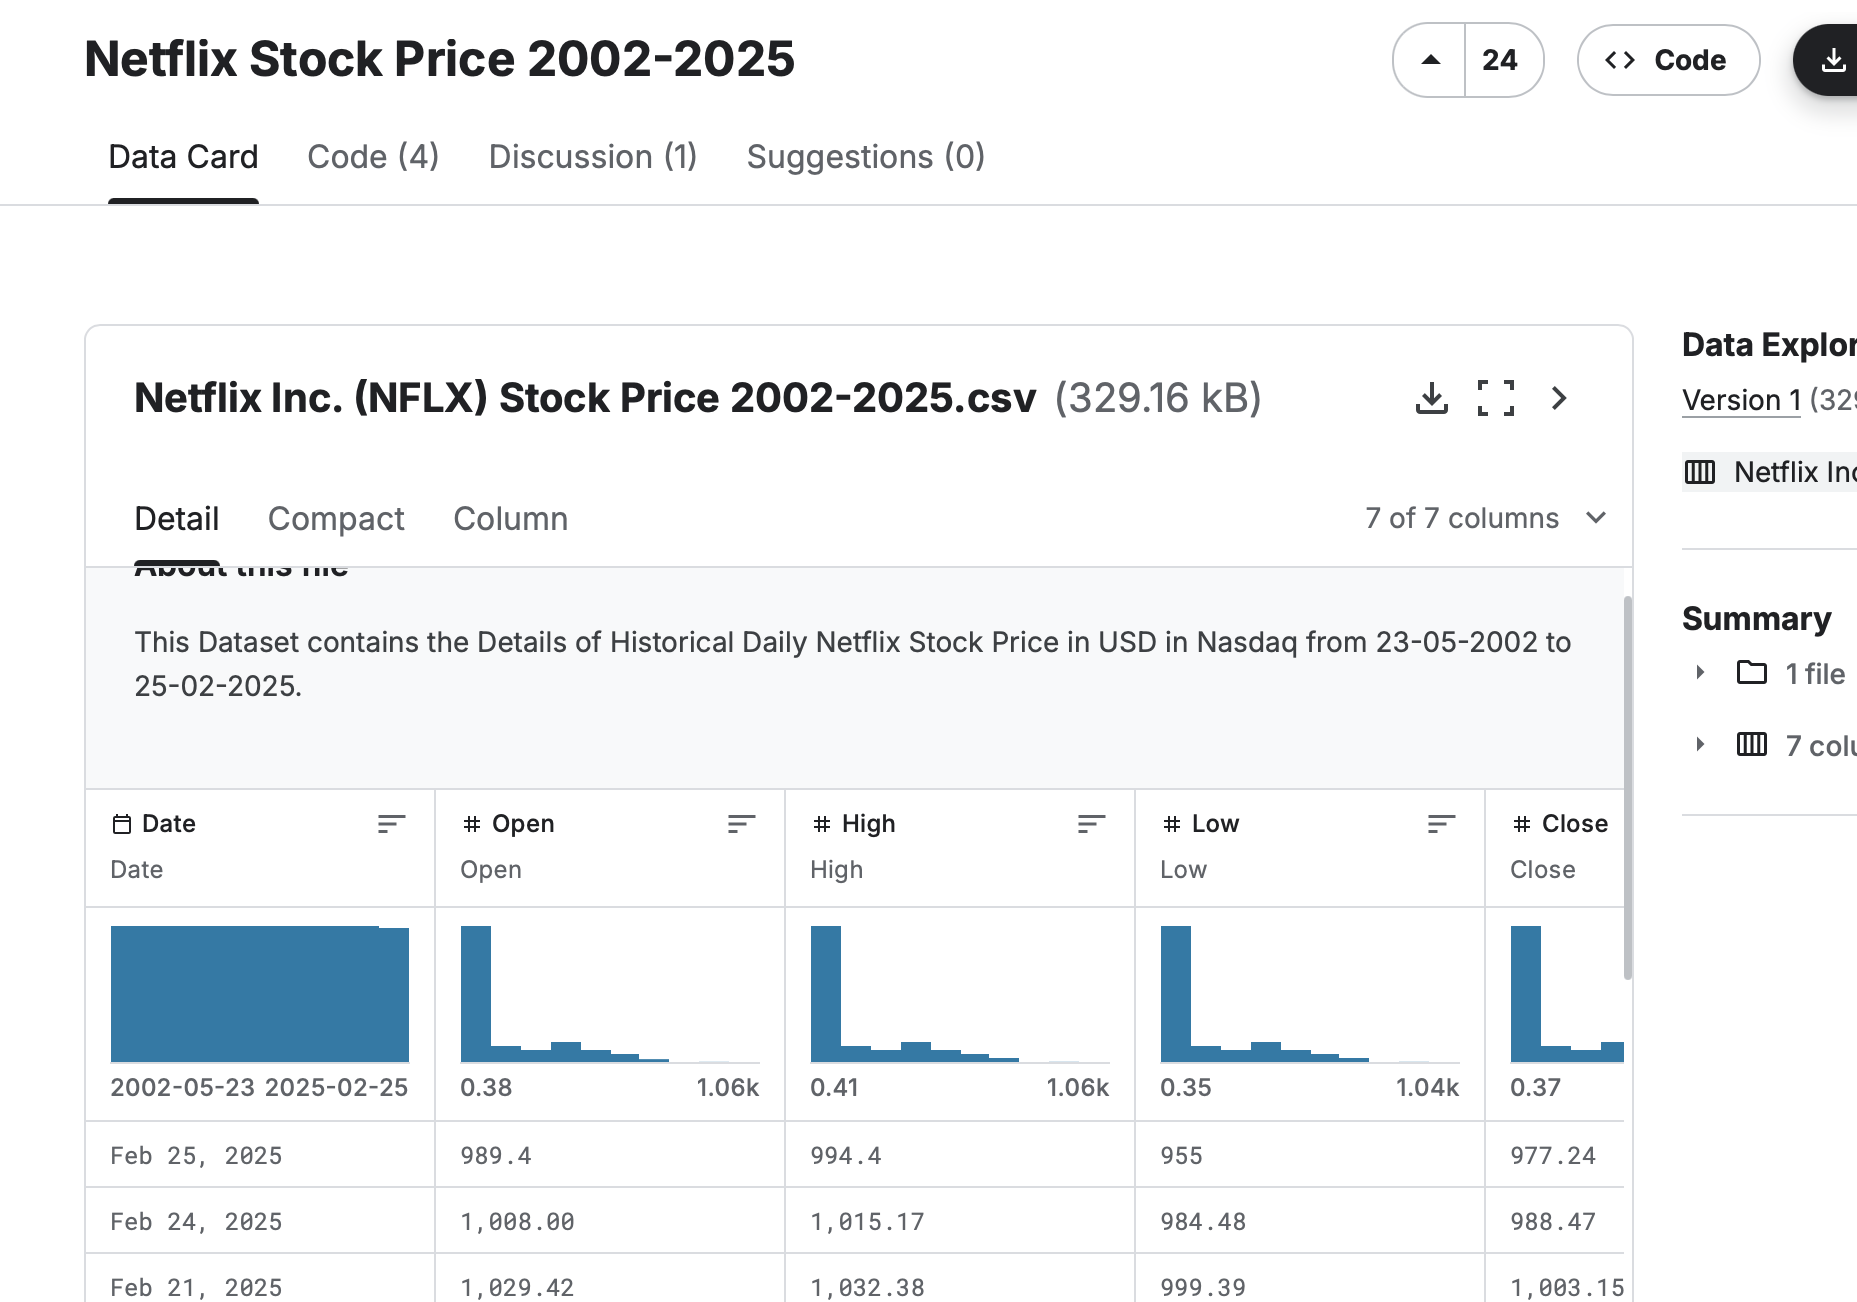
\includegraphics[width=0.5\linewidth]{figure_man/DataSheet.png}

\caption{\tiny Source: \href{https://www.kaggle.com/datasets/samithsachidanandan/netflix-stock-price-2002-2025}{Kaggle Datasets}}
\end{figure}

%\scriptsize
%Based on: \href{https://arxiv.org/abs/1803.09010}{Gebru et al., 2018 — Datasheets for Datasets}
\end{frame}





% \begin{frame}[fragile]{Hidden Features}
% \phantomsection\label{hidden-features}
% \begin{itemize}
% \tightlist
% \item
%   Also known as \emph{confounder variables} (or \emph{mediator
%   variables} in psychology)
% \item
%   Variables that influence your target outcome, but that you
%   didn't measure
% \item
%   Simple example:

%   \begin{itemize}
%   \tightlist
%   \item
%     A customer happiness survey done over 7 days concludes that
%     customers are very unhappy on Fridays and Saturdays
%   \item
%     Hidden feature: There was a rainstorm on these two days
%   \item
%     The hidden feature \texttt{weather}, not the weekday, was
%     responsible for the drop in happiness
%   \end{itemize}
% \item
%   As a more realistic example, data measured over multiple facilities
%   may contain a similar bias, when measurement devices have slight
%   differences in those locations
% \end{itemize}
% \end{frame}

% \begin{frame}{Pipeline}
% \phantomsection\label{pipeline}
% 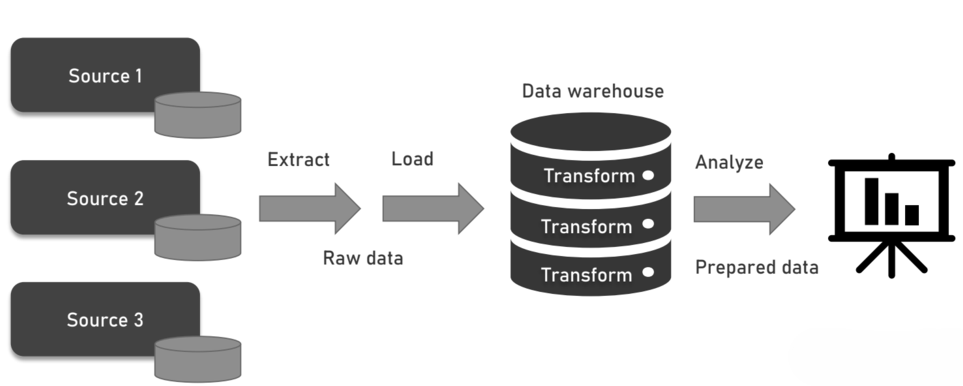
\includegraphics[width = 0.5\linewidth]{figure_man/pipeline.png}
% \begin{itemize}
% \tightlist
% \item
%   You usually need to set up a pipeline to ingest new data and refresh
%   your existing data set regularly.
% \item
%   A pipeline can be

%   \begin{itemize}
%   \tightlist
%   \item
%     batch-based
%   \item
%     streaming or real-time
%   \item
%     a hybrid of these two
%   \end{itemize}
% \end{itemize}
% \textbf{Data Versioning} can make sense, as data changes over time
% \begin{itemize}
% \tightlist
% \item
%   Like version control for code (e.g. Git), it can make sense to have version control for your data sets
% \item
%   \emph{Pachyderm} and \emph{DVC} (Data Version Control) are two
%   versioning tools
% \end{itemize}
% \end{frame}


\begin{frame}{Hidden Complexity in Data}
\phantomsection\label{hidden-complexity}

\vspace{0.5em}
\begin{itemize}
  \item \textbf{Hidden Features:} Unmeasured variables (e.g., confounders) may bias analysis
  \end{itemize}
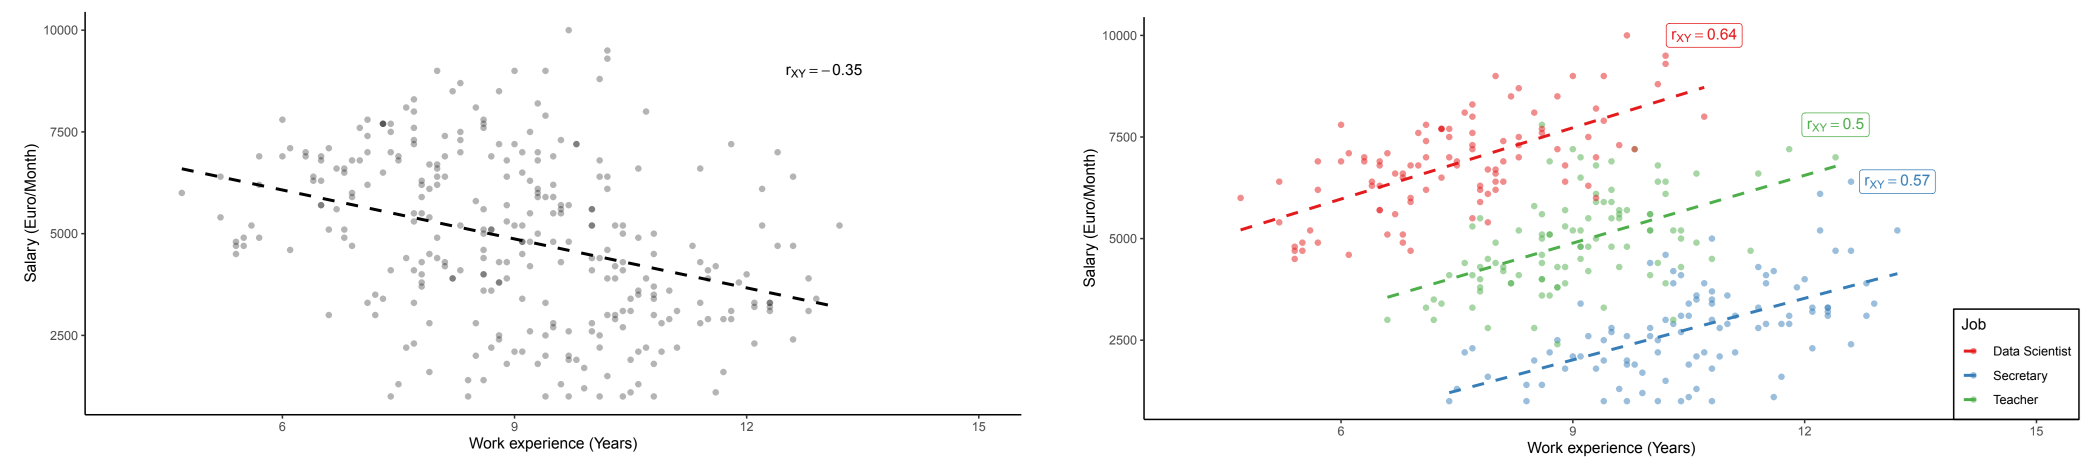
\includegraphics[width = \linewidth]{figure_man/confounder.png}
  % \begin{itemize}
  %   \item Example: Low customer satisfaction on Friday/Saturday may be due to \texttt{weather}, not weekday
  %   \item Real-world case: Subtle biases across facilities due to sensor differences
  % \end{itemize}
  \vspace{-1em}
\begin{itemize}
  \item \textbf{Data Pipelines:} Ensure consistent and reproducible data ingestion
  \begin{columns}[T, totalwidth=\textwidth]
      \begin{column}{0.35\textwidth}
          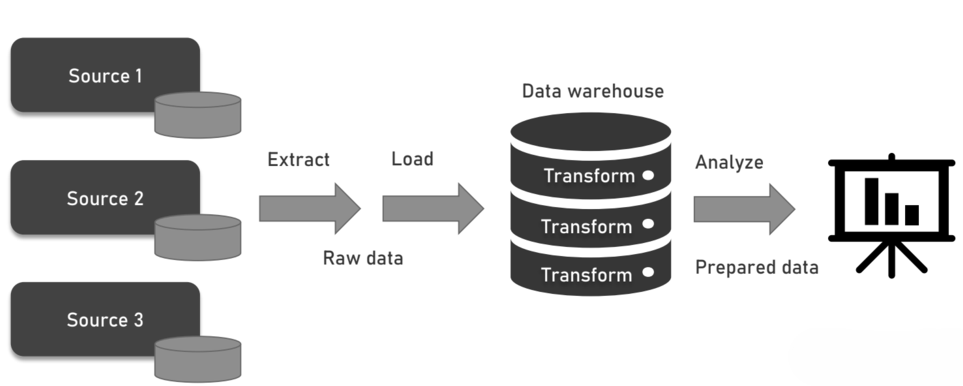
\includegraphics[width = \linewidth]{figure_man/pipeline.png}
      \end{column}
            \begin{column}{0.65\textwidth}
            \begin{itemize}
    \item Can be batch-based, streaming, or hybrid
    \item Should support automated refresh and monitoring
    \item \textbf{Data Versioning} helps track changes over time (e.g., with \texttt{DVC}, \texttt{Pachyderm})
  \end{itemize}
      \end{column}
  \end{columns}

\end{itemize}

\vspace{0.5em}
\textit{Key message: Understanding your data requires both domain awareness and engineering discipline.}
\end{frame}



\begin{frame}{Data Governance and Security}
\phantomsection\label{data-governance-and-security}
\textbf{Key question}: How to keep the data secure, accurate and usable?
\begin{itemize}
\tightlist
    \item \textbf{Integrity}: encure data stays intact when being updated (no duplicates,...)
    \item \textbf{Access}: ensure pipeline allows constant access
    \item establish internal rules for data use
    \item make sure to meet legal requirements such as privacy, anonymization
\end{itemize}
\end{frame}

\begin{frame}{Wrangling, Exploration and Cleaning}
\phantomsection\label{wrangling-exploration-and-cleaning}
\begin{itemize}
\tightlist
\item
  Once you successfully ingested the necessary data, you can begin to
  prepare it for modeling
\item
  This preparation often takes up most of the time in a ML project
\item
  The necessary steps include exploratory data analysis (EDA), data
  wrangling (e.g.~joins) and data cleaning
  \item Sometimes the data you obtain is not yet labeled $\rightarrow$ you need humans (with domain knowledge) to assign labels to your data points
  
\end{itemize}
\end{frame}


\section{3. Modeling}\label{modeling-1}

\begin{frame}{Modeling Steps Overview}
%https://docs.google.com/presentation/d/1RCourH6lXL6sycgT6HbIXWb7rnQvA5HJ/edit?slide=id.p1#slide=id.p1
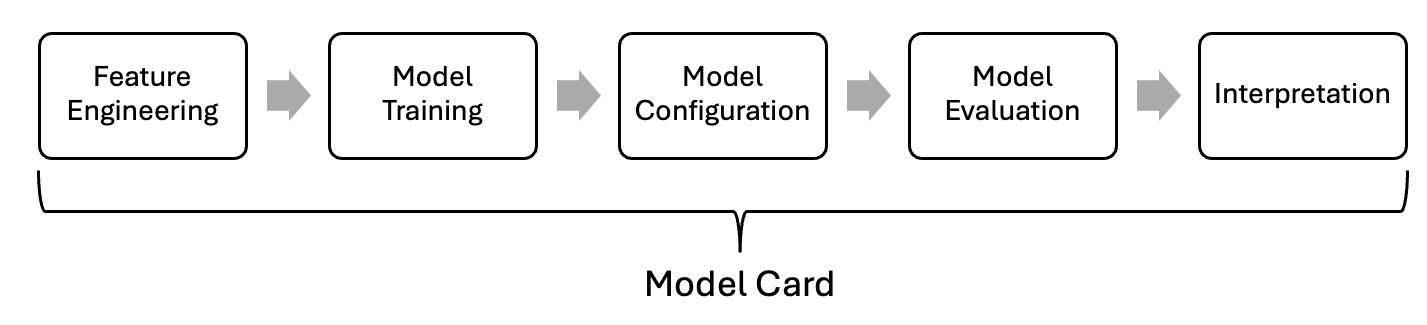
\includegraphics[width = \linewidth]{figure_man/Modelling1.png}
    
\end{frame}

\begin{frame}{Feature Engineering}
\phantomsection\label{feature-engineering}
%https://docs.google.com/presentation/d/1RCourH6lXL6sycgT6HbIXWb7rnQvA5HJ/edit?slide=id.p1#slide=id.p1
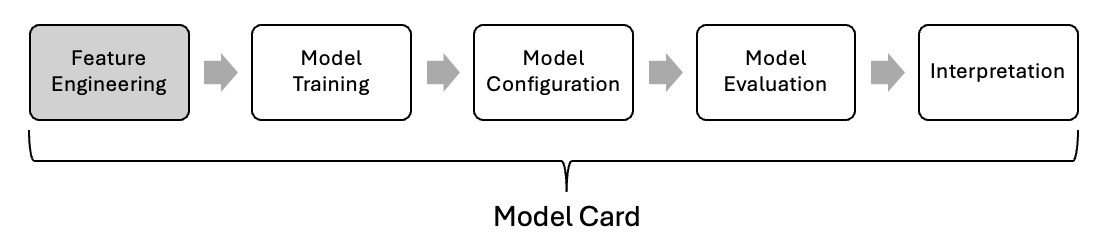
\includegraphics[width = \linewidth]{figure_man/Modelling2.png}
\textbf{Feature Engineering}: selection, aggregation and
  transformation of your raw data to derive meaningful features

Feature Engineering Techniques:

\begin{itemize}
\tightlist
    \item Feature Transformation: Scaling, Log-Transformation, One-hot-encoding
    \item Feature Selection: Feature importance, filtering
    \item Dimensionality Reduction: PCA, t-SNE
    \item Feature Creation: Aggregation, binning, interaction terms
\end{itemize}

Don't overdo it: Including too many useless features introduces
  unnecessary noise into your model\\
  Remember: You have to generate all features for new data.


\end{frame}

\begin{frame}{Model Training}
\phantomsection\label{model-training}
%https://docs.google.com/presentation/d/1RCourH6lXL6sycgT6HbIXWb7rnQvA5HJ/edit?slide=id.p1#slide=id.p1
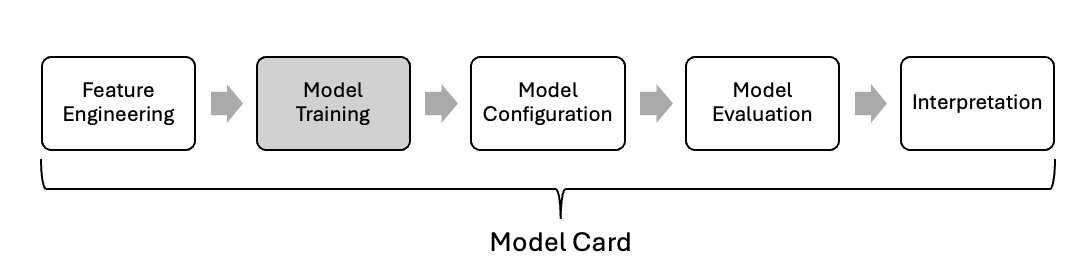
\includegraphics[width = \linewidth]{figure_man/Modelling3.png}
Consider your model training as a scientific experiment:

\begin{itemize}
\tightlist
\item
  Like in a lab experiment, you want to precisely keep track of all
  input parameters

  \begin{itemize}
  \tightlist
  \item
    Data version
  \item
    ML algorithm and hyperparameters
  \item
    Code version (e.g.~a git tag ID)
  \end{itemize}
  \item proceed iteratively:
  \begin{itemize}
\tightlist
\item
  \emph{Start simple}: Quickly create a baseline model
\item
  Then increase the model complexity and verify that each iteration
  improves your target measure
\end{itemize}
\end{itemize}
\end{frame}

\begin{frame}{Model Configuration}
\phantomsection\label{model-configuration}
%https://docs.google.com/presentation/d/1RCourH6lXL6sycgT6HbIXWb7rnQvA5HJ/edit?slide=id.p1#slide=id.p1
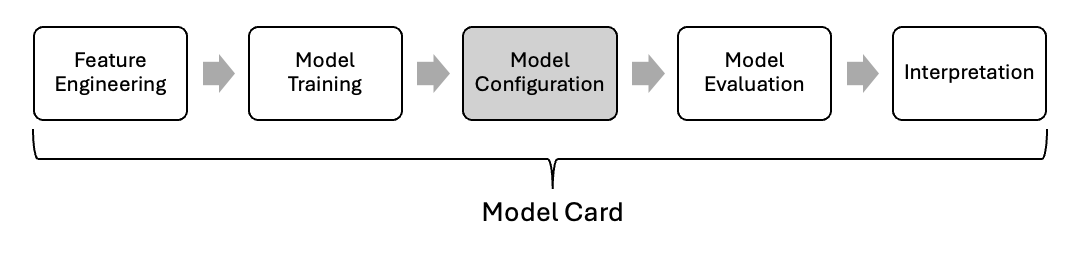
\includegraphics[width = \linewidth]{figure_man/Modelling4.png}
\begin{itemize}
\tightlist
\item
  How do you store a configuration setup you used for a specific
  experiment (model)?\\
  \(\rightarrow\) And how do you store \emph{small} changes to that
  setup?
\item
  This configuration should be stored and clearly readable (i.e.~in
  plain text or json)
\item
  Good tools can help, e.g.~\href{https://hydra.cc}{hydra}
\end{itemize}
\end{frame}

\begin{frame}{Model Evaluation}
\phantomsection\label{model-evaluation}
%https://docs.google.com/presentation/d/1RCourH6lXL6sycgT6HbIXWb7rnQvA5HJ/edit?slide=id.p1#slide=id.p1
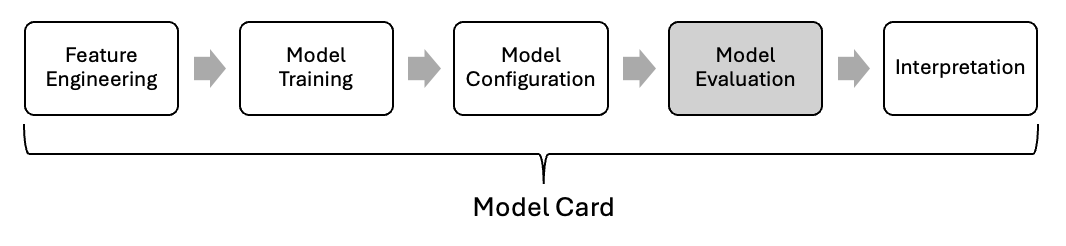
\includegraphics[width = \linewidth]{figure_man/Modelling5.png}
\begin{itemize}
\tightlist
\item
  To select the best model, evaluate based on the
  \textbf{metrics} you predefined
\item Use the test or validation data set according to the validation method predefined
\item
  Besides this performance scoring, you can evaluate your
  model's \textbf{robustness}: How sensitive is it to noise or other pertubations
  and adverserial attacks?

  \begin{itemize}
  \tightlist
  \item
    Add random noise to your dataset and investigate the impact
    on your model's parameters and/or performance
  \end{itemize}
\end{itemize}
\end{frame}

\begin{frame}{Interpretation}
\phantomsection\label{interpretation}
%https://docs.google.com/presentation/d/1RCourH6lXL6sycgT6HbIXWb7rnQvA5HJ/edit?slide=id.p1#slide=id.p1
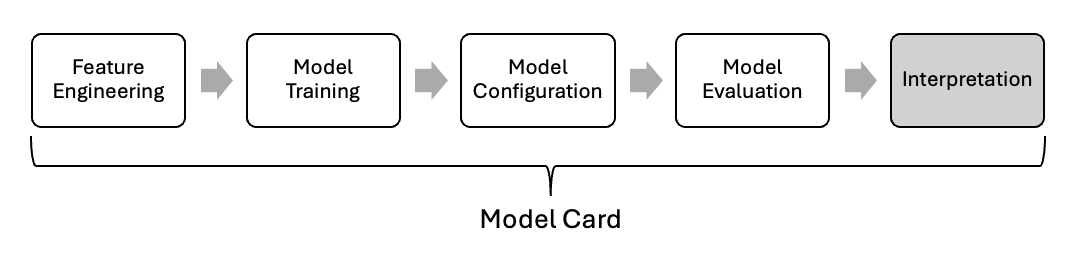
\includegraphics[width = \linewidth]{figure_man/Modelling6.png}
To understand your model better, you can use methods from
  \textbf{Interpretable Machine Learning (IML)}
\begin{itemize}
\tightlist
    \item Feature importances: how much did each feature contribute to the prediction?
    \item uncover potential algorithmic biases:
    \begin{itemize}
    \tightlist
        \item E.g., in October 2018
    \href{https://www.theguardian.com/technology/2018/oct/10/amazon-hiring-ai-gender-bias-recruiting-engine}{world
    headlines reported} about an Amazon AI recruiting tool that favored
    men. Amazon's model was trained on biased data that were skewed
    towards male candidates. It has built rules that penalized resumes
    that included the word ``women's''.
    \end{itemize}
\end{itemize}
\end{frame}

\begin{frame}{Model Cards}
\phantomsection\label{model-cards}
%https://docs.google.com/presentation/d/1RCourH6lXL6sycgT6HbIXWb7rnQvA5HJ/edit?slide=id.p1#slide=id.p1
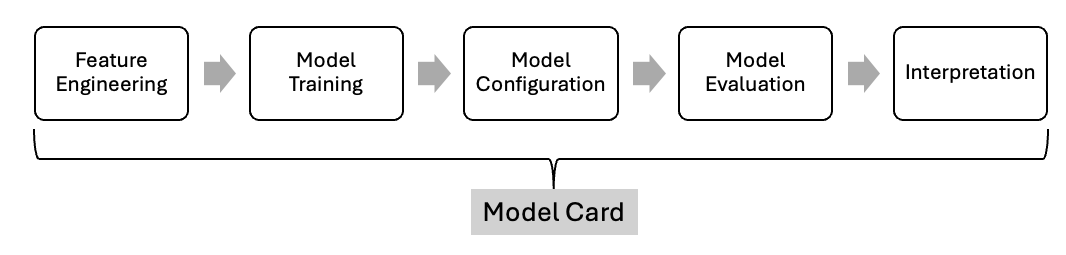
\includegraphics[width = \linewidth]{figure_man/Modelling7.png}
\textbf{Model Card}: documentation for the model similar to Datasheet for data, includes:
\begin{itemize}
\tightlist
    \item Performance characteristics
    \item Intended use cases
    \item Unrecommended usage
\end{itemize}
See also: \href{https://arxiv.org/pdf/1810.03993.pdf}{Model Cards for
  Model Reporting}
\end{frame}

\section{4. Model Governance}\label{model-governance-1}

\begin{frame}{Model Governance}
\phantomsection\label{model-governance-2}
\begin{quote}
Developing and deploying ML systems is relatively fast and cheap, but
maintaining them over time is difficult and expensive.
~\href{https://papers.nips.cc/paper/5656-hidden-technical-debt-in-machine-learning-systems.pdf}{Hidden
Technical Debt in ML Systems}
\end{quote}
\end{frame}

\begin{frame}{Model Governance}
\phantomsection\label{model-governance-3}
\begin{itemize}
\tightlist
\item
  Model Governance includes the \textbf{people, processes and
  technologies} needed to manage and protect your ML model.
\item it ensures easy maintenance and possibilities for adaption
\item
  Two extremes have to be avoided:

  \begin{itemize}
  \tightlist
  \item
    \textbf{Repression} by too many standards, rules, and controlling
  \item
    \textbf{Chaos} by too much speed, freedom, creativity and change
  \end{itemize}
\end{itemize}
\end{frame}

\begin{frame}{Model Governance}
    Model Governance Steps are:
    %https://docs.google.com/presentation/d/1RCourH6lXL6sycgT6HbIXWb7rnQvA5HJ/edit?slide=id.p1#slide=id.p1
    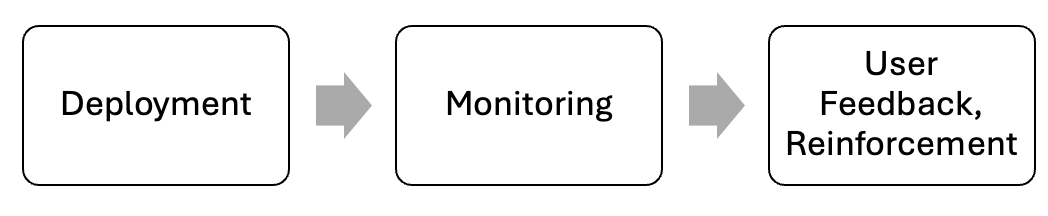
\includegraphics[width = \linewidth]{figure_man/Model Governace.png}
\end{frame}

\begin{frame}{Deployment}
\phantomsection\label{deployment}
%TODO include graphics on deployment strategies
\textbf{Deployment}: make model accessible to users (humans or other programs)
\begin{itemize}
\tightlist
\item
  You can deploy your model in different ways:

  \begin{itemize}
  \tightlist
  \item
    \textbf{One-off}: If you only need your model trained once (or very
    rarely), train it by hand and push it to production
  \item
    \textbf{Batch}: With batch training, you constantly (e.g.~weekly)
    update your model with a new batch of data (e.g.~this week's new
    contracts)
  \item
    \textbf{Real-time}: Some models are very time-critical and need to
    be updated continously on a stream of data.
  \end{itemize}
\item If you retrain and update your model frequently, it makes sense to have some model \textbf{versioning}
\begin{itemize}
\tightlist
    \item \href{https://mlflow.org/}{MLflow} is an open source platform for ML
  lifecycle management that includes a model registry
\end{itemize}
\end{itemize}
\end{frame}


\begin{frame}{Monitoring}
\phantomsection\label{monitoring}
\textbf{Monitoring}: detect possible problems in productive use and provide fixes:

\begin{itemize}
\tightlist
    \item Pipeline bugs
    \item \textbf{Data drift}: data distribution changes
    \begin{itemize}
    \tightlist
        \item Example: You train an image classifier on animal pictures taken in
    summer, and then winter comes and images start containing snow.
    \item Another possibility is that your \emph{target} evolves, and now
  includes new categories or new value ranges in case of a continuous
  target
  \item Remedy: Enough of the new data needs to be labeled to introduce the
  model to the new classes, and the model needs to be retrained
    \end{itemize}
    \item \textbf{Concept drift}: interpretation of data changes
    \begin{itemize}
    \tightlist
        \item Example: A classification problem into “high blood pressure”, and the cutoff
for “high blood pressure” changes from 140mmHg to 135mmHg.
        \item Remedy: Your affected old data needs to be relabeled and the model retrained
    \end{itemize}
\end{itemize}

\end{frame}



\begin{frame}{User Feedback, Reinforcement}
\phantomsection\label{user-feedback-and-acceptance}
At the end of the project, you will:
\begin{itemize}
\tightlist
    \item \textbf{System Validation}: Ask for customer feedback if the model
    and data pipeline meet their needs
    \item \textbf{Project handover}: Transfer the project to the team that
    will run your system in production
\end{itemize}
\end{frame}

\begin{frame}{User Feedback, Reinforcement}
\phantomsection\label{user-feedback-and-acceptance}

You can also include \textbf{Feedback Loops/ Reinforcement}:

\begin{itemize}
\tightlist
\item
  \textbf{Direct feedback loops}: A model may influence the selection of
  \emph{its own} future training data.

  \begin{itemize}
  \tightlist
  \item
    Example: Netflix influences which movies it recommends to certain
    viewers, and it will then use (only) these movies as future training
    data
  \end{itemize}
\item
  \textbf{Hidden feedback loops}: Here, \emph{two systems} influence
  each other \emph{indirectly} through the world.

  \begin{itemize}
  \tightlist
  \item
    Example: Flash crashes that occur because many trading algorithms
    sell at the same time and augment each others fear
  \end{itemize}
\end{itemize}
\end{frame}



\section{Best Practices for Competition Success}
%TODO graphics with overview over steps
\begin{frame}{Step 1: Understand the Problem Statement}
\begin{itemize}
  \item \textbf{Clarify Objectives \& Business Impact}: Determine whether it’s a classification or regression task, the domain context, and what “success” looks like.
  \item \textbf{Target Variable}: Understand how the target is defined and distributed.
  \item \textbf{Constraints \& Permissions}: External data limits, privacy, or regulatory issues.
  \item \textbf{Action Points}:
    \begin{itemize}
      \item Annotate key requirements and assumptions.
      \item Research the domain for feature ideas.
      \item Restate the problem in your own words to ensure clarity.
    \end{itemize}
\end{itemize}
\end{frame}

\begin{frame}{Step 2: Study the Evaluation Metric}
\begin{itemize}
  \item \textbf{Metric Matters}: Each competition or project has a specific metric (e.g., F1-score, AUC-ROC, RMSE), which guides how you tune and compare models.
  \item \textbf{Classification vs. Regression Metrics}:
    \begin{itemize}
      \item Accuracy, F1-score, AUC-ROC, and Log Loss for classification.
      \item RMSE, MAE, R\textsuperscript{2} for regression.
    \end{itemize}
  \item \textbf{Optimization Direction}: Decide if you must maximize or minimize the metric; some metrics (e.g., AUC-ROC) may need a proxy loss for training.
  \item \textbf{Action Points}:
    \begin{itemize}
      \item Simulate prediction changes to see impact on the metric.
      \item If allowed, implement custom losses aligned to the competition metric.
    \end{itemize}
\end{itemize}
\end{frame}

\begin{frame}{Step 3: Perform an Initial Data Analysis (EDA)}
\begin{itemize}
  \item \textbf{Data Profiling}: Summarize shape, basic statistics, feature and target distribution.
  \item \textbf{Quality Checks}: Identify missing values, outliers, or suspicious patterns; confirm no hidden data leakage.
  \item \textbf{Train-Test Shift}: Check if train and test set differ significantly in their feature distributions.
  \item \textbf{Action Points}:
    \begin{itemize}
      \item Use tools like Pandas Profiling or Sweetviz for automated EDA.
      \item Document anomalies or domain-specific oddities.
      \item Examine correlations, scatter plots, and histograms.
    \end{itemize}
\end{itemize}
\end{frame}

\begin{frame}{Step 4: Develop a Baseline Model}
\begin{itemize}
  \item \textbf{Why a Baseline?} A simple model (e.g., Logistic Regression, Decision Tree) gives you a reference performance.
  \item \textbf{Pipeline Check}: Make sure that data loading, preprocessing, and validation splits are correct.
  \item \textbf{Diagnostics} : Analyze misclassifications/ residuals to spot improvement areas.
  \item \textbf{Action Points}:
    \begin{itemize}
      \item Start with a naive or default-parameter model.
      \item Use cross-validation to assess reliability.
      \item Record baseline metrics to quantify future gains.
    \end{itemize}
\end{itemize}
\end{frame}

\begin{frame}{Step 5: Set Up a Robust Validation Strategy}
\begin{itemize}
  \item \textbf{Importance of Validation}: Avoid overfitting or a single random split.
  \item \textbf{Common Methods}:
    \begin{itemize}
      \item K-Fold (balanced data).
      \item Stratified K-Fold (imbalanced classes).
      \item Time-Based or Group Splits (time series, repeated measures).
    \end{itemize}
  \item \textbf{Action Points}:
    \begin{itemize}
      \item Match validation approach to the final test scenario.
      \item Keep a holdout set for final checks.
      \item Use consistent folds across experiments to compare fairly.
    \end{itemize}
\end{itemize}
\end{frame}

\begin{frame}{Step 6: Feature Engineering and Data Preprocessing}
\begin{itemize}
  \item \textbf{Missing Data}: Mean/median imputation, advanced methods, or flags.
  \item \textbf{Encoding Categorical Variables}: One-hot/ target/ frequency enc. (leakage?!).
  \item \textbf{Scaling \& Transformations}: Normalize or log-transform skewed features, especially for sensitive models (SVMs, neural nets).
  \item \textbf{New Features}: Time-based, domain knowledge, interactions (e.g. ratios).
  \item \textbf{Action Points}:
    \begin{itemize}
      \item Add features in small batches and track validation changes.
      \item Use scikit-learn Pipelines to avoid leakage.
      \item Consider dimensionality reduction if feature space is large.
    \end{itemize}
\end{itemize}
\end{frame}

\begin{frame}{Step 7: Select and Tune Models Strategically}
\begin{itemize}
  \item \textbf{Model Choices}:
    \begin{itemize}
      \item Tree-based ensembles (XGBoost, LightGBM, CatBoost) for tabular data.
      \item Neural networks for large-scale or unstructured data.
      \item Simple linear/logistic models can still compete with good feature engineering.
    \end{itemize}
  \item \textbf{Hyperparameter Tuning}:
    \begin{itemize}
      \item Grid Search, Random Search, Bayesian Optimization.
      \item Early stopping and regularization (L1, L2) to avoid overfitting.
    \end{itemize}
  \item \textbf{Action Points}:
    \begin{itemize}
      \item Track experiments (MLflow, Weights \& Biases, or spreadsheets).
      \item Start with defaults and refine gradually.
      \item Use IML tools (SHAP, permutation importance) for feature insights.
    \end{itemize}
\end{itemize}
\end{frame}

\begin{frame}{Step 8: Track Experiments and Iterate}
\begin{itemize}
  \item \textbf{Experiment Logging}: Keep detailed records of data versions, hyperparams, code revisions.
  \item \textbf{Error Analysis}: Study misclassifications and residuals to guide feature tweaks.
  \item \textbf{Iterative Improvements}:
    \begin{itemize}
      \item Refine features, adjust validation, revisit transformations.
      \item Maintain a “changelog” for each iteration.
    \end{itemize}
  \item \textbf{Action Points}:
    \begin{itemize}
      \item Automate repeated tasks (submissions, data prep).
      \item Prune ineffective ideas swiftly.
      \item Ensure reproducibility (version control, environment snapshots).
    \end{itemize}
\end{itemize}
\end{frame}

\begin{frame}{Step 9: Understand the Leaderboard and Avoid Overfitting}
\begin{itemize}
  \item \textbf{Public vs. Private Leaderboard}: Public boards use only part of the test set—overfitting leads to dramatic rank changes later.
  \item \textbf{Submission Strategy}:
    \begin{itemize}
      \item Rely mainly on internal validation.
      \item Keep a private holdout to confirm final performance.
    \end{itemize}
  \item \textbf{Leaderboard Shakeups}: Watch for big changes when private scores are revealed; it often indicates overfitting to the public set.
  \item \textbf{Action Points}:
    \begin{itemize}
      \item Limit minor tweaks solely to improve a public rank.
      \item If a jump seems suspicious, re-check data handling for leakage.
    \end{itemize}
\end{itemize}
\end{frame}

\begin{frame}{Step 10: Collaborate and Learn from Others}
\begin{itemize}
  \item \textbf{Study Top Solutions}: Many winning approaches are documented in blog posts or Kaggle discussions.
  \item \textbf{Teamwork}:
    \begin{itemize}
      \item Collaboration brings diverse perspectives and model ensembling.
      \item Share code and features for synergy.
    \end{itemize}
  \item \textbf{Community \& Networking}:
    \begin{itemize}
      \item Discussion forums reveal dataset quirks, best practices.
      \item Local meetups or online communities keep you updated.
    \end{itemize}
  \item \textbf{Action Points}:
    \begin{itemize}
      \item Document and share your findings.
      \item Adapt others’ ideas carefully—validate them on your own splits.
      \item Engage with peers for new tools and techniques.
    \end{itemize}
\end{itemize}
\end{frame}

\begin{frame}{Final Advice}
\begin{itemize}
  \item \textbf{Start Simple, Then Iterate}: Don’t jump into complex models, get a solid baseline.
  \item \textbf{Prioritize Validation}: A robust validation strategy prevents nasty surprises.
  \item \textbf{Log Everything}: Document transformations, parameters, and model versions.
  \item \textbf{Aim for Generalizable Solutions}: Don’t just chase leaderboard scores—focus on reproducibility and reliability.
\end{itemize}
\end{frame}



\end{document}
